\chapter{面向交易执行优化的孪生对抗自体再生方法}

% 兼容局部浮动体分组控制：若主文件已加载 placeins，则使用正式 \FloatBarrier；若未加载，则不影响编译。
\providecommand{\FloatBarrier}{}

\section{问题的提出}

\subsection{交易执行中的滑点风险与市场冲击成本}

% 在完成了从宏观资产配置（第 2 章）、中观因子建模（第 3 章）到微观形态分类（第 4 章）的预测体系构建后，本章将研究焦点下沉至算法交易的最终执行环节——VWAP（成交量加权平均价格）滑点控制\cite{almgren2001optimal,madhavan2002vwap}。在现代高频交易环境中，预测精度与经济价值之间往往存在非单调性悖论：一个在统计误差上表现优异的模型，若在流动性枯竭或趋势反转的关键节点发生方向性误判，可能放大执行滑点与市场冲击成本\cite{berkowitz1988total,cartea2015algorithmic}。

在完成投资组合管理、高维金融因子建模与时序结构识别之后，交易系统已经分别形成了资产配置对象、因子依据和时机判断。然而，这些信号只有进入真实下单路径后，才能转化为可实现收益。本章进一步进入对冲基金交易决策流程中的交易执行优化环节，重点讨论交易执行路径如何优化的问题\cite{almgren2001optimal}。交易执行优化并不是前序模型的附属步骤，而是决定模型信号能否在市场摩擦、流动性约束和冲击成本条件下落地的独立环节。成交量加权平均价格作为机构投资者最广泛采用的执行基准之一，其核心目标在于将大额订单的实际成交均价控制在市场成交量加权均价附近，从而最小化对市场价格的冲击并降低信息泄露风险。对本文而言，成交量调度不是单纯的执行技巧，而是检验前序资产配置、因子依据和时序结构信号能否在真实市场中稳定落地的关键接口：一旦订单时间分布与市场流动性状态发生错配，前序模型形成的交易判断就可能在执行层转化为滑点、冲击成本和异常回撤。因此，本章将成交量加权平均价格执行作为具体场景，研究如何通过孪生对抗自体再生方法优化执行路径、过滤异常信号并降低执行偏差，使交易执行优化成为连接模型信号与真实成交结果的关键环节\cite{madhavan2002vwap}。

在现代高频交易环境中，预测精度与经济价值之间往往存在非单调性悖论：一个在统计误差上表现优异的模型，若在流动性枯竭或趋势反转的关键节点发生方向性误判，可能放大执行滑点与市场冲击成本。这一悖论的根源在于，统计损失函数与经济损失函数之间存在结构性错位。实证研究表明，交易成本的真实构成远比表面的买卖价差复杂，隐性成本往往占据主导地位\cite{berkowitz1988total}。在此背景下，如何在预测精度之外纳入执行成本与流动性约束，成为算法交易系统设计的重要问题。Cartea 与 Jaimungal 在随机控制框架下系统论证了执行算法的设计需将市场状态的动态反馈纳入优化目标，静态的预设执行计划在非平稳市场条件下将面临严重的次优性\cite{cartea2015algorithmic}。

从市场微观结构角度看，滑点并不是由单一价格误差造成的，而是买卖价差、订单簿深度、信息不对称与短时流动性共同作用的结果。市场微观结构综述表明，交易制度、报价机制和订单流结构会直接影响成交价格的形成过程\cite{Ananth2000Market}。进一步的实证研究也说明，市场微观结构变量不仅决定交易成本的大小，还会改变交易策略在不同市场状态下的可执行性\cite{hasbrouck2007empirical}。因此，对成交量加权平均价格执行而言，关键并不是在任意时点都追求更低预测误差，而是在有限时间窗口内识别哪些流动性片段更适合承接订单。流动性交易理论指出，执行者需要在等待流动性与立即成交之间权衡，否则容易将大额订单暴露为额外冲击成本\cite{huberman2005optimal}。

进一步看，成交量加权平均价格执行并不是单纯的价格预测问题，而是一个同时受到成交量分布、订单拆分路径与市场微观结构约束的序列决策问题。为避免在问题提出部分过早展开公式推导，本节先从交易含义上说明其核心关系：执行者需要在给定总订单量和有限执行窗口内，将订单量分配到不同时间片，并使实际执行均价尽量贴近市场成交量加权平均价格。若订单切片与真实成交量分布不匹配，执行均价就会偏离基准价格，形成滑点损失；若这种偏离在非平稳行情中持续扩大，前序模型形成的交易信号就可能在成交层面被抵消。相应的成交量加权平均价格、执行量约束、实际成交均价与滑点损失等形式化表达，将在5.3.4节结合执行层修复目标集中给出。算法交易研究也指出，执行算法的价值取决于信号、成本和市场反馈之间的协调，而不是单独依靠某一类预测器完成全部决策\cite{2014Algorithmic}。

基于上述分析，本章将交易执行优化中的关键问题凝练为：如何把前序形成的交易信号转化为稳定的订单执行路径，如何在成交量预测误差、流动性错配和市场冲击之间建立动态约束，以及如何在候选执行信号退化时及时触发校验与修复。也就是说，本章方法需要真正回应的不是“能否预测成交量”，而是“能否在预测成交量—执行路径—滑点控制—崩溃修复之间形成可运行的闭环”。后文提出的孪生对抗自体再生方法正是围绕这一闭环展开。

\subsection{现有执行基准的结构性困境}

从交易执行优化视角看，现有执行基准的局限并不仅在于成交量曲线预测不够精确，而在于其通常缺乏对执行偏差、流动性错配和异常滑点的独立识别能力。静态成交量曲线假定历史成交分布可以为未来下单路径提供稳定参考，但真实市场中的流动性峰谷、突发冲击和参与者行为变化会不断改变执行环境。当执行器仍按固定模板下单时，上游资产、因子和时序结构信号可能在成交层被转化为价格冲击、成交滞后和滑点扩散。因此，本节讨论的结构性困境，本质上是现有执行框架缺少对执行路径的动态校验、异常过滤和持续调整能力。孪生对抗自体再生方法的引入，正是为了使执行系统能够在候选信号进入真实下单路径前完成校验与再平衡，从而服务于交易执行路径优化任务。

由此，本章的问题提出可以进一步归纳为三点：第一，执行层需要将前序信号映射为可执行的订单时间分布，而不能只保留离线预测结果；第二，执行模型需要识别成交量预测与真实流动性之间的偏离，避免订单集中落入不利时间片；第三，当模型组内出现同步退化或局部对抗失衡时，需要通过自体再生机制恢复执行系统的差异化校验能力。上述三点分别对应后文的动态调度器、孪生校验结构和跨组修复流程。

传统成交量加权平均价格算法以历史成交量分布为主要依据，其优势在于规则清晰、易于执行，但这一设定也意味着执行路径较容易受到历史均值曲线的约束。相关研究已经从竞争性分析角度讨论了在线决策在未知环境中的基准参照问题，为理解静态执行基准的局限提供了理论背景\cite{kakade2004competitive}。在真实市场中，成交量峰谷、订单簿深度和短时冲击会随市场状态变化而快速调整，执行器若缺少实时校验环节，就可能在低流动性阶段被动成交，或在价格不利区间放大交易冲击。

这一问题在高频交易环境下更加明显。市场微观结构研究表明，高频成交过程中的报价调整、订单到达和流动性供给会显著改变短周期价格形成机制\cite{goodhart1997high}。因此，执行基准不能只被理解为一条平均成交量曲线，而应被理解为一个需要随成交环境持续校验的动态参照系。已有改进成交量加权平均价格的研究也说明，仅依赖静态曲线难以充分适配真实日内成交形态，执行路径需要结合市场状态进行修正\cite{bialkowski2008improving}。这为本章后续引入动态调度器提供了直接动因。

与此同时，现有执行模型还面临预测精度与经济价值不一致的问题。早期关于预测评价的研究已经指出，统计精度提升并不必然意味着经济价值提升\cite{leitch1991economic}。对应到交易执行任务中，均方误差较低的成交量预测模型，并不一定能够降低滑点和冲击成本；真正决定执行质量的，往往是关键时间片上的流动性识别、异常成交过滤和转折状态下的路径调整能力。因此，本章关注的不是单纯降低成交量预测误差，而是使执行模型能够识别何时应当信任预测、何时应当降低敞口或触发自体再生。

从模型结构看，生成式和多模型方法为刻画复杂市场状态提供了新的工具，但也带来模型同步退化和局部共识幻觉的风险。多生成器生成对抗网络的研究表明，多个生成主体可以扩展样本模式覆盖范围，但不同主体之间仍需要有效的差异化约束和稳定训练机制\cite{ghosh2018multi}。若执行系统只叠加多个候选预测器而缺少独立校验机制，多个模型可能在同一类异常行情中同时失效。孪生对抗自体再生方法的核心作用，正是通过复制、配对与分化过程保留候选模型之间的可比较性，并在偏离累积到阈值时触发替换和短程修复，避免执行路径被单一退化信号长期主导。

综上，现有执行基准的结构性困境并不是单一预测精度不足，而是静态基准、经济价值错位和模型退化风险共同作用下形成的执行层稳定性问题。后文将围绕这一问题，进一步说明孪生对抗自体再生机制如何在执行前校验、异常过滤和动态调度中发挥作用。



\section{相关工作}

成交量加权平均价格执行优化的相关研究，通常围绕成交量预测、最优执行、市场冲击控制与执行路径校验展开。已有研究在执行基准设计、成交量曲线建模和市场状态表征方面积累较多，但对候选执行信号进入真实下单路径前的独立校验、异常过滤与动态再平衡讨论仍相对不足。因此，本节不再只围绕单一执行基准的精度展开，而是结合执行基准、预测价值错位、市场状态表征、生成式金融序列建模、模型互校验和多智能体系统等研究，说明孪生对抗自体再生方法的引入背景。

从执行基准研究看，成交量加权平均价格之所以被广泛采用，是因为它能够把大额订单拆解为与市场成交节奏相匹配的时间路径，并为交易成本评价提供相对稳定的参照。相关研究从理论层面讨论了成交量加权平均价格执行策略在特定市场冲击假设下的最优性条件，为理解该类基准的适用前提提供了基础\cite{kato2014vwap}。不过，这种最优性通常依赖于成交量分布、价格冲击函数和流动性状态的稳定假设；一旦日内成交结构发生偏移，单纯跟随历史均值曲线就可能放大滑点风险。进一步的最优性研究也表明，成交量加权平均价格执行并不是脱离约束条件的普遍最优策略，其有效性需要结合市场冲击、成交量过程和执行约束共同理解\cite{kato2016optimality}。因此，第五章关注的重点不是重新证明成交量加权平均价格基准本身的有效性，而是讨论执行系统如何在基准失效风险出现时进行动态校验和路径修正。

从成交量预测研究看，日内成交量比例并非完全随机，仍可通过历史成交形态、市场状态和短周期价格信息进行建模。近期关于日内成交量估计的研究表明，成交量曲线预测可以为订单拆分和执行节奏调整提供信息基础\cite{lee2024ive}。但是，对本文而言，成交量预测只是执行优化链条中的一个环节。即使预测曲线在均值意义上较为准确，关键时间片上的局部偏差仍可能造成集中成交、冲击成本上升或执行滞后。金融时间序列的经验事实也提示，收益分布、波动聚集和厚尾特征会使局部市场状态偏离常规均值假设\cite{Cont2001Empirical}。因此，孪生对抗自体再生方法并不只追求成交量预测误差最小化，而是进一步关注候选执行信号在进入下单路径前是否需要经过独立校验和再平衡。

从预测价值与执行价值的关系看，金融预测结果在统计指标上的改善并不必然转化为执行绩效改善。在非平稳市场中，预测模型的样本外表现和经济价值往往会随评价窗口、市场状态和交易成本假设变化而改变\cite{rossi2021forecasting}。这意味着执行模块不能把上游预测结果视为稳定输入，而需要在进入成交路径前重新判断其成本敏感性和风险暴露。进一步地，面向交易目标的训练研究也提示，若损失函数不能反映实际经济后果，模型可能在统计精度提升的同时放大执行端偏差\cite{zhou2024two}。因此，本章把预测输出视为待校验的候选信号，而不是直接下单依据。

从市场状态表征看，深度时序模型和订单簿建模方法增强了系统对短周期流动性、订单流不平衡和价格微结构的刻画能力。多变量时序预测研究说明，跨变量依赖和时间选择信息能够帮助模型识别不同阶段的状态变化\cite{lim2021temporal}。这类方法为执行系统理解市场状态提供了上游表征基础，但仍主要服务于预测任务；对于第五章而言，更关键的是将状态信息转化为下单路径中的校验、过滤与修复机制。以限价订单簿深度学习建模为代表的研究说明，深度模型能够从盘口形态中提取对短期价格变动有用的结构信息\cite{zhang2019DeepLOB}。这类研究为执行层理解市场微观结构提供了重要工具，但其目标通常仍偏向价格方向预测或状态识别。交易执行优化还需要进一步回答：当候选信号与真实流动性不一致时，系统如何发现偏离、如何过滤异常信号，以及如何避免退化模型持续主导下单路径。

从生成式金融序列建模看，对抗生成框架为刻画复杂数据分布提供了重要工具。生成对抗网络通过生成器与判别器之间的博弈过程学习数据分布，为金融场景中的序列生成和分布模拟提供了基础方法参照\cite{goodfellow2014generative}。不过，执行优化并不只需要生成“看起来合理”的市场路径，还需要判断这些路径是否会误导真实下单行为。面向金融时间序列的生成式研究进一步说明，生成模型可以在一定程度上复现收益序列的统计特征，为压力场景构造和样本扩展提供可能\cite{wiese2020quant}。这类研究对执行优化有启发意义，但若缺少执行前校验，生成样本中的局部偏差仍可能被下游调度器放大为实际滑点。

围绕多模型对抗与市场情景模拟的研究，也为本章的孪生校验思想提供了间接参照。多判别器生成框架通过引入多个判别视角增强对生成样本的约束，说明单一判别器并不总能充分识别复杂样本空间中的偏差\cite{nguyen2017dual}。金融市场生成器相关研究则从市场冲击和压力情景角度讨论了生成模型在金融模拟中的作用，为理解极端执行环境下的候选路径退化提供了补充视角\cite{kondratyev2019market}。这一视角说明，执行优化中的生成式建模不能停留在样本扩展层面，还需要进一步检验候选路径在流动性收缩、冲击成本放大和成交量分布偏移条件下是否仍具有可执行性。换言之，生成模型提供的是可能的市场情景，而孪生校验机制需要判断这些情景中的候选下单路径是否会被异常波动或局部结构误导。
此外，生成式智能体研究强调，在复杂交互环境中，主体行为与反馈机制会共同影响系统状态演化\cite{santoro2022generative}。这些研究共同说明，执行系统若希望在非平稳、高噪声市场中保持稳定，不能只依赖单一预测或单一判别结果，而需要保留可比较、可校验的候选主体。

多生成器和多智能体生成模型进一步揭示了模型多样性与校验机制之间的关系。多生成器对抗模型通过引入多个生成主体缓解模式单一问题，为理解候选执行信号的多样性维护提供了方法启发\cite{madgan2018multiagent}。但是，多主体结构本身并不能自动保证执行安全；如果缺少异常识别和自体再生机制，多个模型也可能在相同市场偏差下同步退化。由此，第五章采用孪生对抗自体再生方法，并不是简单增加模型数量，而是通过复制、配对和分化建立执行前的冗余校验路径。

从异常识别和模型互校验角度看，深度互学习的相关研究表明，通过在多个网络之间建立对称的监督信号，可以有效提升单个模型的泛化能力并抑制过拟合\cite{zhang2018dml}。这一思想说明，模型之间的相互约束可以成为提升稳健性的来源。相关研究还表明，在集成判别器框架中引入轻量化异常检测模块，能够在保持计算效率的同时增强系统对退化信号的过滤能力\cite{xie2022lightweight}。这些工作提示，执行系统在面对候选成交量信号退化或判别边界偏移时，不宜只依赖单一预测器，而应引入可比较、可替换的校验结构。基于这一研究脉络，后文将孪生对抗自体再生方法用于执行路径的异常识别、信号校验和动态再平衡。

从多智能体视角看，交易执行天然具有多主体博弈特征。Markov Games 将多智能体强化学习形式化为多个决策主体共同影响状态转移的框架，为理解执行系统中的竞争与反馈提供了基础\cite{littman1994markov}。在此基础上，执行系统中的候选模型可以被理解为具有不同判别边界和风险偏好的主体，其输出需要在统一执行约束下接受比较。多智能体强化学习综述也指出，在非平稳环境中，智能体间的协作、竞争和信用分配会直接影响系统稳定性\cite{busoniu2008comprehensive}。这与本章的设计逻辑一致：执行系统不能只依赖单一预测器，而应保留多个可比较、可替换、可再生的候选主体。量化金融中的机器学习、深度学习和强化学习综述也指出，交易算法通常需要同时处理预测、仓位、成本和风险四类目标\cite{sahu2023overview}。因此，本章将执行优化理解为多目标约束下的动态校验过程，而不是单一预测模型的输出转换。

与“构造单一最优预测器”的思路不同，已有执行基准、成交量预测、市场状态表征、生成式金融序列建模、互学习、异常检测与多智能体研究共同指向一种更适合执行优化的思路：执行系统需要保留可比较的候选主体，并在偏离出现时具备识别和再平衡能力。后文提出的“复制—配对—分化”自体再生逻辑，正是在这一研究脉络下形成的执行前校验机制。

上述研究为交易执行优化提供了成交量预测、最优执行、多智能体学习和异常检测等基础，但对执行信号进入真实下单路径前的独立校验与自体再生讨论仍不充分。围绕这一不足，下文将依次展开自体再生机制的结构设计、触发逻辑、跨组自体再生程序以及动态成交量加权平均价格调度器，并结合真实高频数据检验其在减少滑点、适应市场微观结构差异及稳定执行路径方面的表现。

\section{孪生对抗自体再生方法}

本节从交易执行优化任务出发说明孪生对抗自体再生方法的结构与运行逻辑。与只追求成交量预测误差最小化的执行模型不同，本章将该方法设计为执行前校验与动态再平衡过程：先由多智能体候选池生成可比较的执行信号，再利用孪生结构进行配对校验，并通过偏离统计识别局部失衡；当跨组约束满足时，系统触发参数镜像、替换和短程对抗微调。由此，模型设计的重点不在于额外叠加预测器，而在于形成“候选生成—孪生校验—偏离识别—执行优化”的连续过程，并将“预测成交量—执行路径—滑点控制—崩溃修复”的因果链落实到模型结构中。

\subsection{机制引入动因与执行风险修复需求}

第 4 章完成时序结构识别后，模型已经能够为交易系统提供相对结构化的趋势信号，但该信号进入实际执行环节后仍会受到成交量分布、订单簿深度和短时流动性的约束。若执行层只按照静态成交量曲线或单一预测结果下单，时序结构识别阶段得到的信号可能在成交过程中被滑点、冲击成本和局部流动性断裂抵消。因此，执行层面对的不是简单预测误差，而是前序信号能否在市场微观结构约束下稳定兑现的问题。

因此，本章引入孪生对抗自体再生方法，其动因在于为成交量加权平均价格执行任务增加一层执行前校验与动态再平衡能力。这里的执行风险修复，主要指交易执行优化过程中对异常滑点、候选信号退化和局部对抗失衡的主动校验与动态调整。该方法将异常滑点、候选模型退化和局部对抗失衡统一视为可观测的偏离状态，并通过孪生校验、跨组替换和短程微调完成再平衡。在这一处理下，执行系统不再只是接收上游模型输出的末端模块，而是具备执行路径识别、过滤和调整能力的执行优化模块。

\subsection{复制—配对—分化的自体再生逻辑}

为应对执行信号在非平稳市场下可能出现的退化问题，本章提出孪生对抗自体再生方法，并将其嵌入成交量加权平均价格执行任务之中。该方法并不重新设计投资组合管理、高维金融因子建模或时序结构识别模型，而是在执行信号进入最终下单路径之前，通过复制、配对与分化三个步骤构建独立校验机制。复制用于保留当前最优或相对稳定的模型状态，为后续执行路径再平衡提供参数参考；配对用于构建功能相近但判别边界不完全相同的孪生模型，使系统能够通过双重校验识别候选执行信号的异常偏离；分化则通过独立训练和短程对抗微调避免孪生体完全同化，从而保留异常检测能力。三者共同作用，使执行层偏差能够从外部滑点表现转化为内部可比较、可触发、可优化的状态。

多智能体系统研究表明，当多个学习主体共享环境并相互影响时，系统性能往往不再等同于单个模型性能的简单叠加\cite{stone2000multiagent}。在金融市场中，主体之间的相互影响更为明显，基于智能体的计算金融研究长期将市场视为由异质交易者共同演化形成的复杂系统\cite{lebaron2006agent}。因此，本章采用“复制—配对—分化”的设计，并不是为了增加模型数量本身，而是为了让系统在执行前保留可比较、可分化的判别边界。

\begin{figure}[htbp]
\centering
% \includegraphics[width=\linewidth]{figures/chap4/intro (cropped).pdf}
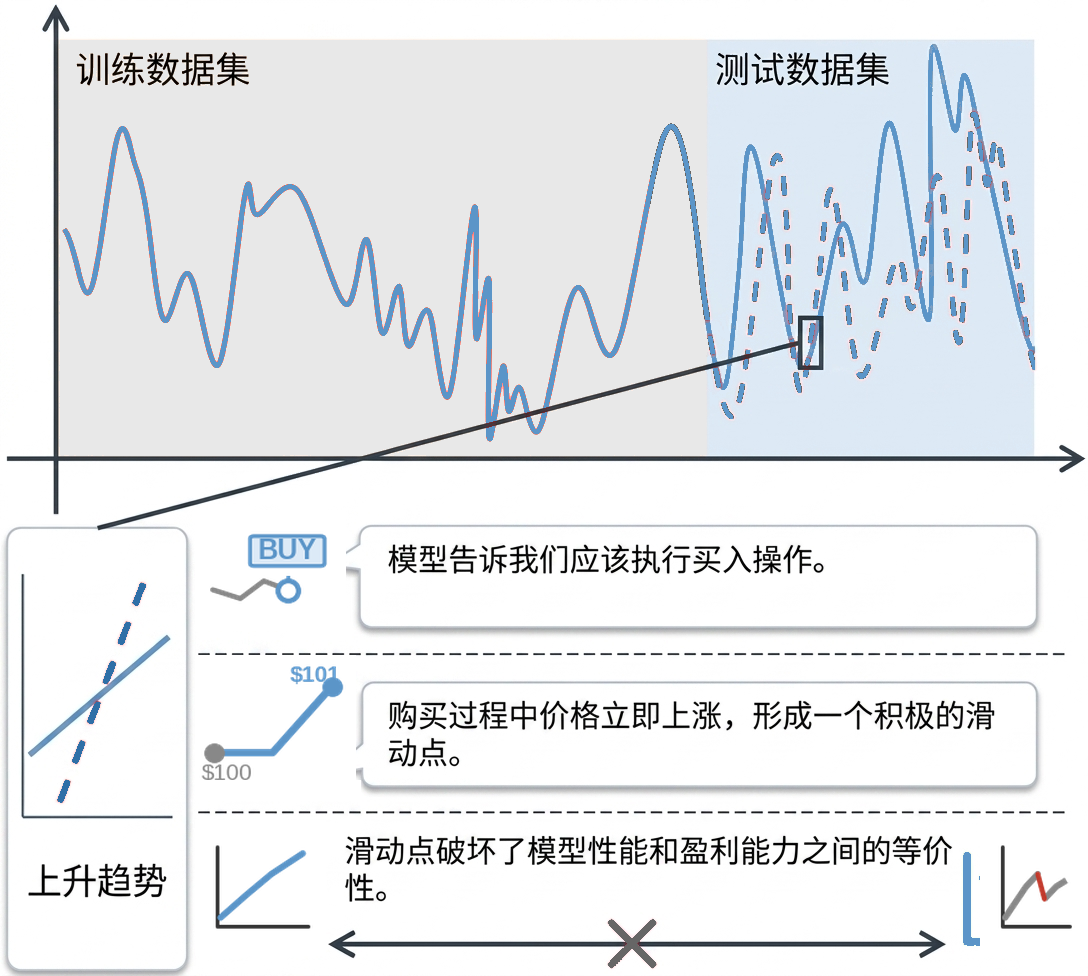
\includegraphics[width=\linewidth]{figures/chap6/图5.1改.png}
\caption{下单执行流程}
\label{fig:intro_new}
\end{figure}

图\ref{fig:intro_new}展示了从候选生成、孪生校验到最终下单执行的总体流程。该流程表明，本章方法并不替代前述模块，而是作为执行前的校验环节，对上游输出进行独立校验与风险过滤。

\begin{figure}[htbp]
    \centering 
    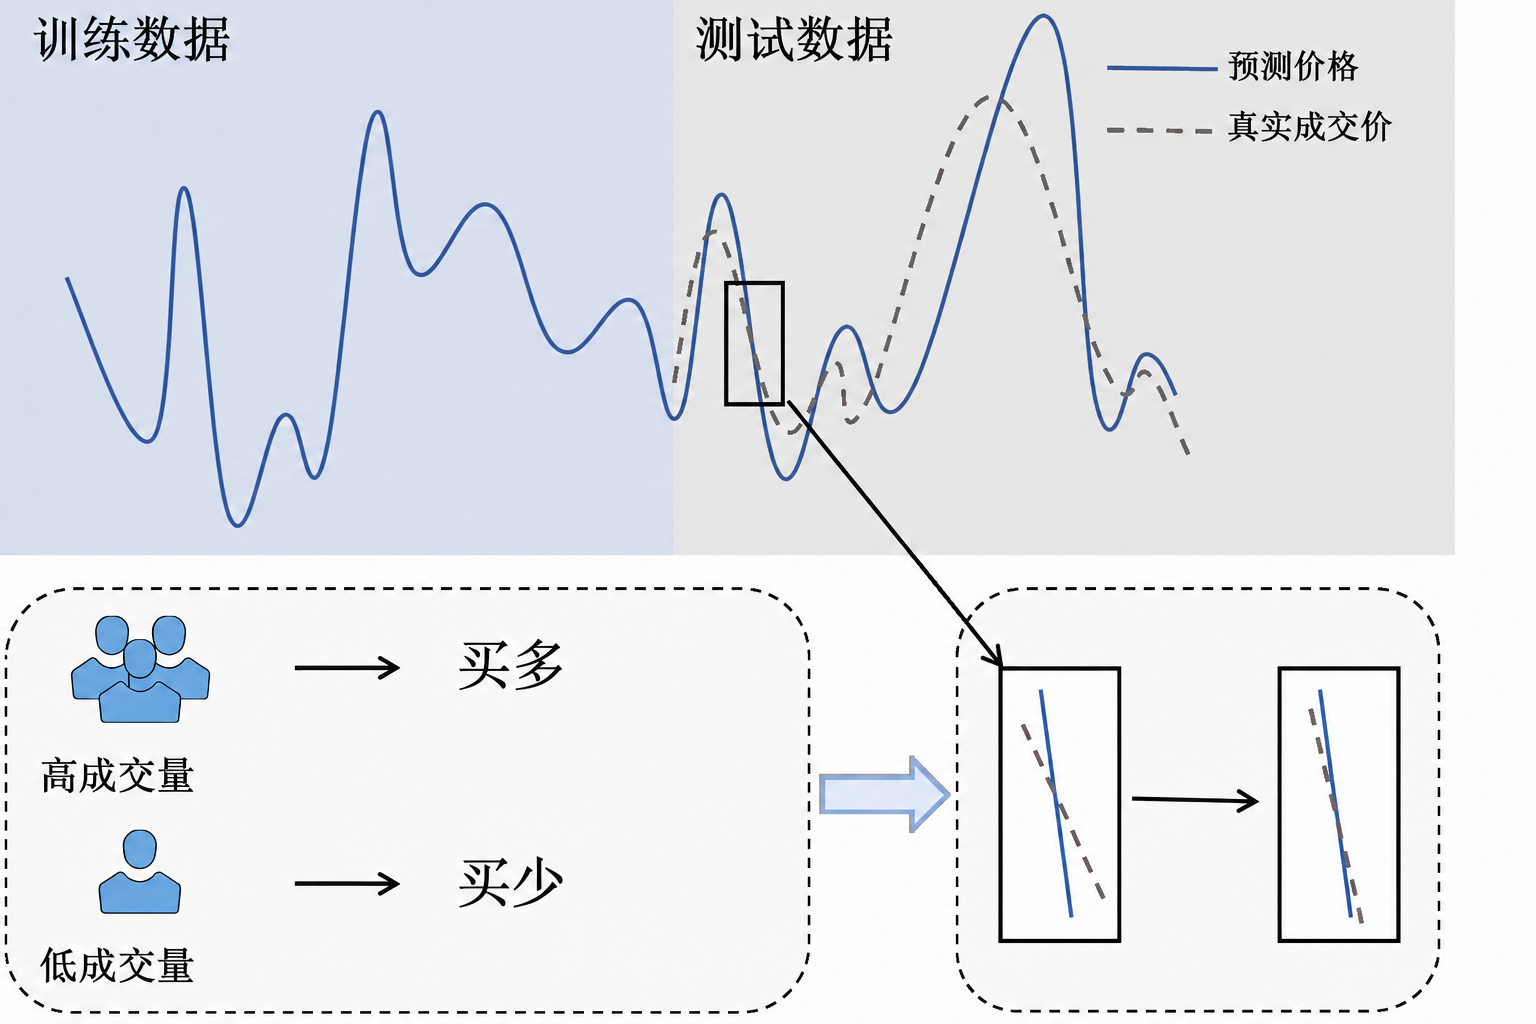
\includegraphics[width=0.8\textwidth]{figures/chap6/图5.2改.png} 
    \caption{孪生对抗自体再生方法在交易执行优化中的任务定位}
    \label{fig:vwap_task_new}
\end{figure}

图\ref{fig:vwap_task_new}给出了本章方法在多智能体对抗体系中的任务位置。其重点不在于追求单次预测最优，而在于判断系统能否在高噪声、厚尾与分布迁移环境中维持相对稳定的执行状态。

在此基础上，本章引入并系统性研究基于该机制减少滑点的方法（基于自体再生机制的成交量加权平均价格执行方法）。其基本思想是：以两个具有独立判别边界的成对子系统，对通过赛马场竞争机制选出的候选执行信号进行一致性认证；当任一子系统的模型偏离累计达到预设阈值时，触发替换与再平衡程序。这样，系统不再依赖单一判别器的一次性判断，而是在“双轨校验”中保留足够的容错空间。

\begin{figure}[htbp]
    \centering
    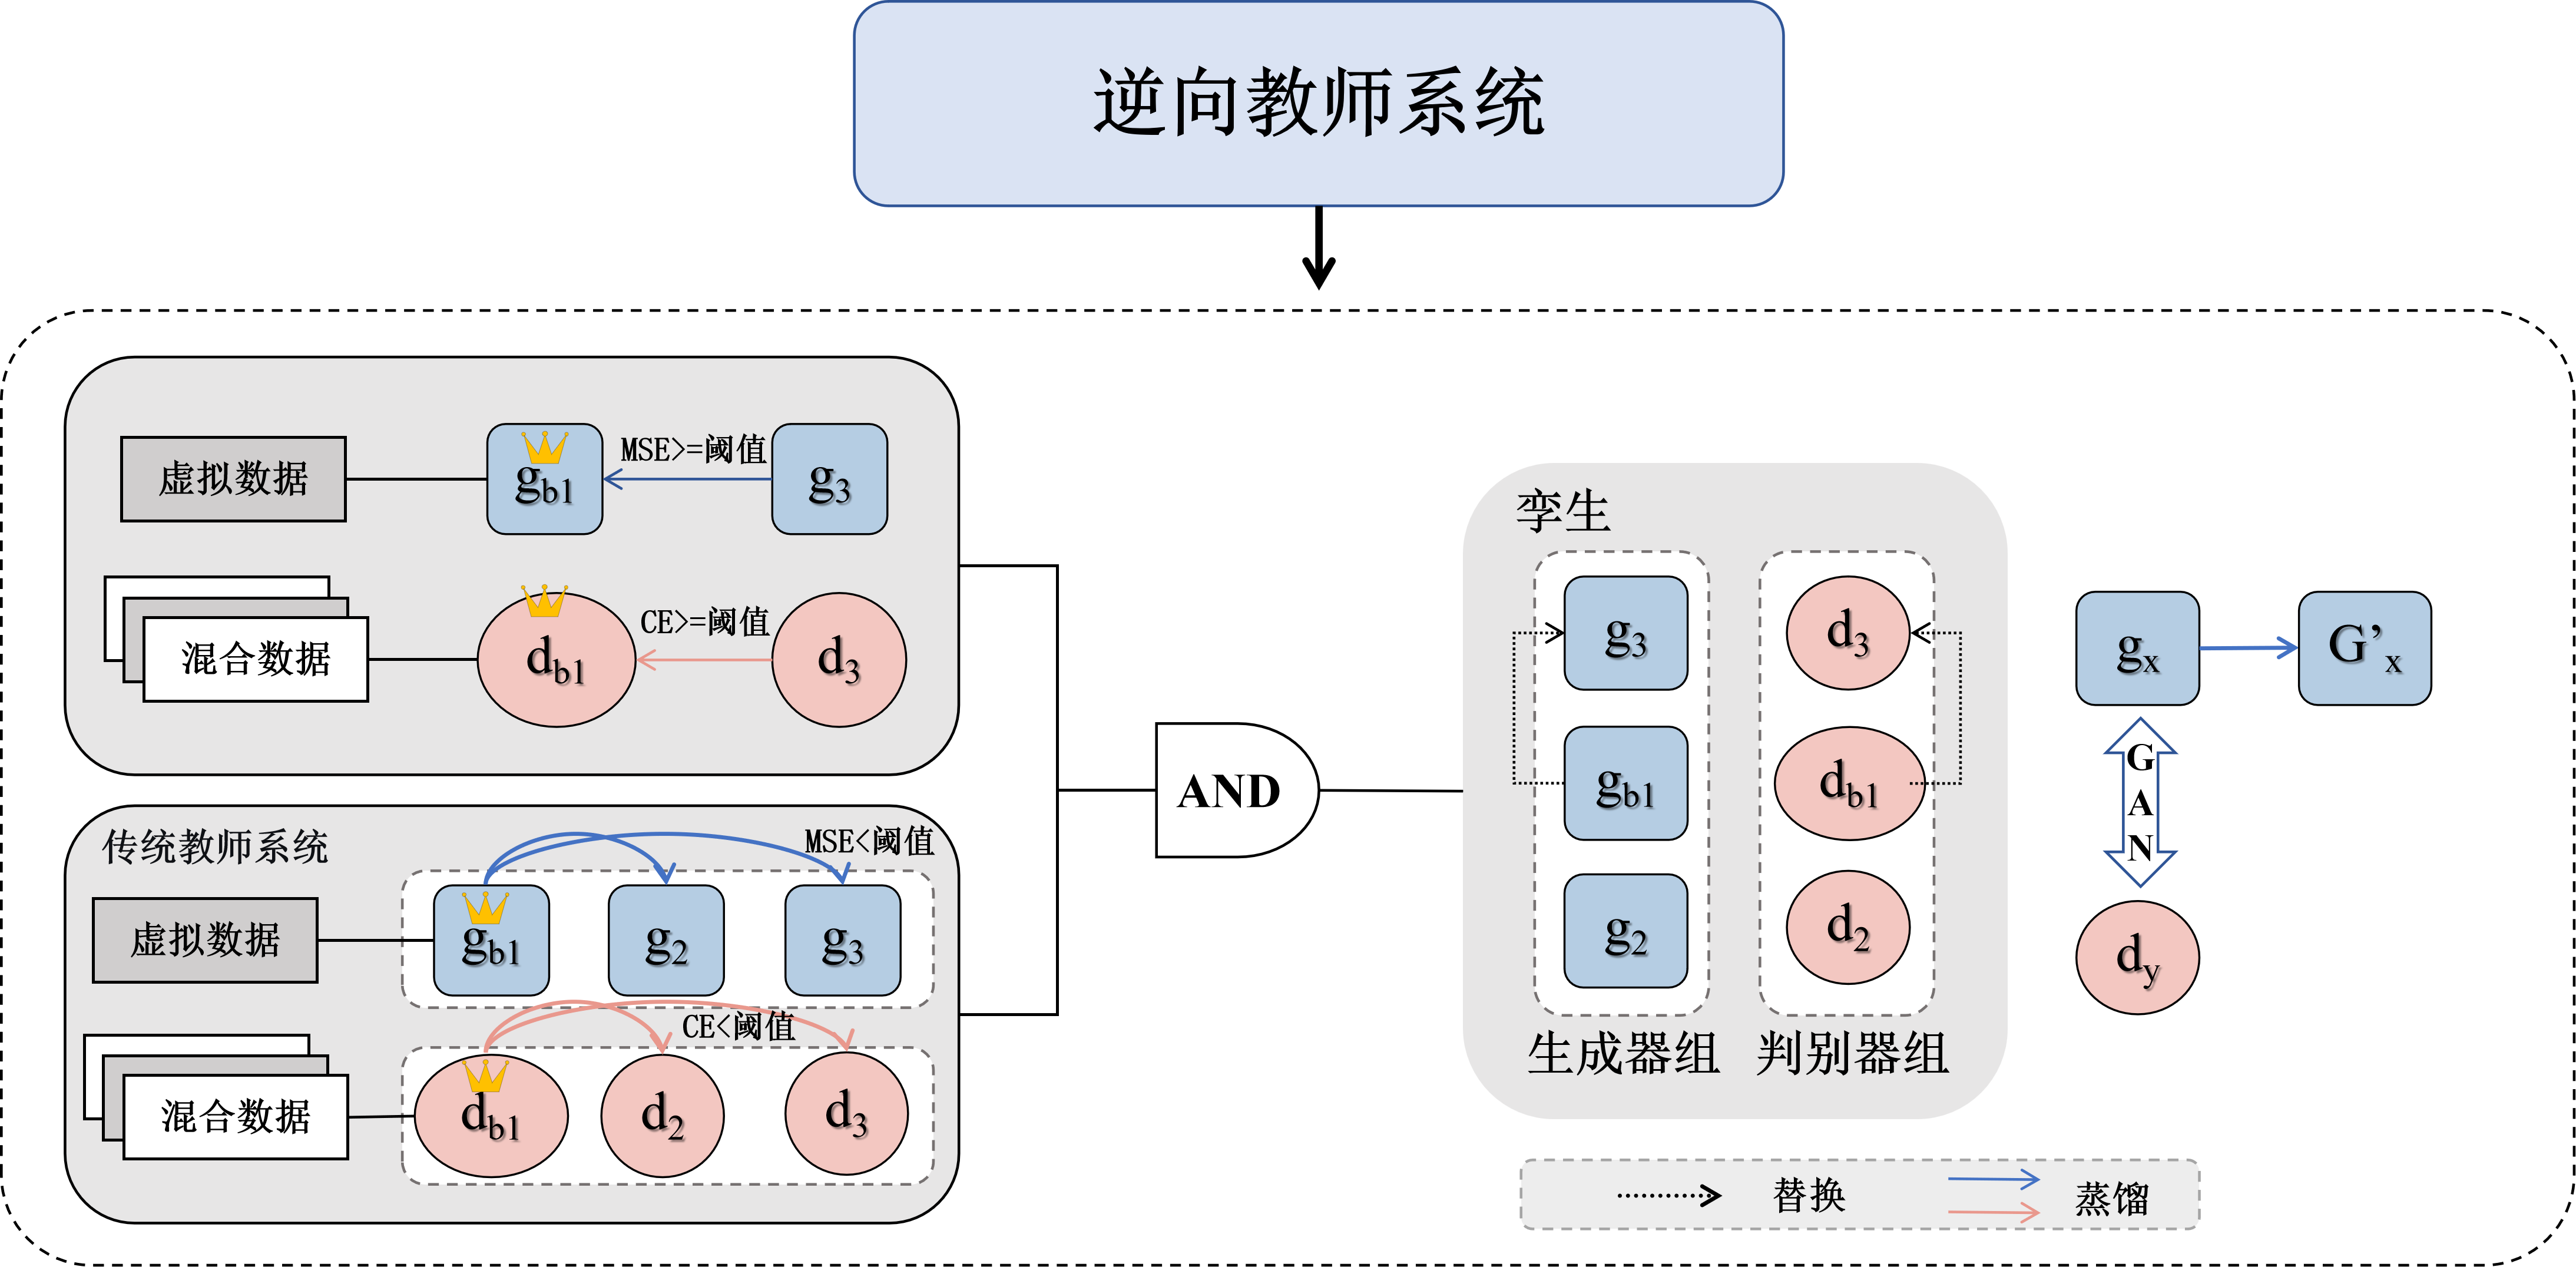
\includegraphics[width=0.8\textwidth]{figures/chap6/孪生对称.png}
    \caption{孪生对抗训练流程示意图}
    \label{fig:VWAP-workflow-new}
\end{figure}

图\ref{fig:VWAP-workflow-new}展示了孪生对抗训练流程。与传统单判别器结构相比，该流程通过复制优胜个体、为其建立独立对偶、并在后续训练中使其重新分化，使系统在保留高质量参数起点的同时避免完全同质化。这种“复制—配对—分化”逻辑，本质上是一种带有恢复能力的对抗冗余设计。

合作式多智能体学习研究指出，多主体系统若缺少明确的分工和反馈机制，容易出现学习效率下降或策略趋同的问题\cite{panait2005cooperative}。对本章而言，这一问题不能简单理解为模型数量不足，而应理解为复制后的候选主体能否形成可验证的功能差异。若孪生体在相同输入下持续给出趋同判断，复制过程只会增加冗余计算，难以形成对异常成交路径的有效校验。因此，后续自体再生机制需要在继承有效参数的同时，保留主体之间的差异化分工。

在金融投资任务中，多智能体组合管理系统也体现出通过分工学习不同资产或策略视角的价值\cite{lee2020maps}。这一思路映射到交易执行层，意味着孪生体不应只是重复给出同一执行判断，而应在相同订单约束下保留不同的风险过滤边界，用于比较候选信号是否会放大滑点、集中下单或触发异常成交路径。对做市任务的强化学习研究则表明，交易主体需要在收益、库存风险与成交概率之间持续权衡，这与本章执行层的风险过滤逻辑具有一致性\cite{spooner2018market}。因此，该机制中的复制并非简单克隆，而是在保留有效参数的同时重新建立差异化校验路径。

\subsection{跨组修复流程与崩溃抑制机制}

自体再生方法的设计动机，集中体现在对模型退化的可测量化处理上。尽管上游多智能体框架已能提升候选信号多样性与知识共享能力，执行层仍可能面临三类风险：生成器预测严重失真、判别器失效导致错误放行，以及模型组内同步退化并形成局部最优。为此，本章将“异常偏离”显式定义为可统计、可触发、可再平衡的数学对象。跨组修复流程的作用，是在局部模型组发生偏离时避免异常执行信号继续进入订单拆分与真实下单路径。与简单删除异常模型不同，本章将修复过程设计为受约束的再平衡过程：只有当偏离统计持续超过阈值，且其他模型组仍保持相对稳定时，系统才触发参数镜像或跨组替换；替换完成后，还需要通过短程对抗微调恢复新成员与原有群组之间的差异化边界。这样可以避免修复动作本身造成新的模型同质化或级联崩溃。对交易执行优化而言，模型崩溃并不只是训练过程中的技术问题，而会表现为错误成交量分布、异常订单切片或过度集中下单。跨组修复流程通过偏离统计与参数镜像机制，将这些潜在执行偏差前置到模型内部识别，从而降低异常信号直接转化为滑点和冲击成本的概率。

强化学习基础研究表明，序列决策问题通常通过状态、动作和奖励之间的反馈关系优化长期目标\cite{Mnih2015HumanlevelCT}。在交易执行任务中，这一思想可以进一步转化为对订单切片、成交概率和执行成本之间关系的动态优化；早期强化学习最优执行研究已经将交易执行明确表述为可通过市场反馈学习的决策问题\cite{nevmyvaka2006reinforcement_acm}。因此，本章将偏离统计量写入触发规则，是为了让执行风险在模型内部形成可追踪的反馈信号。

首先，对生成器或判别器引入偏离统计量。设每个成员的性能以均方误差或交叉熵表征，则生成器 $G_i$ 在时间步 $t$ 相对于当前最优生成器 $G_{\mathrm{best}}$ 的偏离度记为：
\begin{equation}
\Delta_i^{(t)} = \mathcal{L}(G_i, G_{\mathrm{best}}).
\label{eq:delta_stat_new}
\end{equation}
在训练过程中，若偏离度超过阈值 $\epsilon$，则对该成员累计一次超阈值计数：
\begin{equation}
N_i = \sum_{t=1}^{N} \mathbf{1}\left[ \Delta_i^{(t)} > \epsilon \right].
\label{eq:deviation_count_new}
\end{equation}
相应地，在更细粒度的实现中，生成器与判别器分别采用以下距离统计：
\begin{equation}
\delta_i^{(t)} = \mathrm{MSE}\left( G_i^{(t)}(x)_{:, -1, \text{close}},\; G_{\mathrm{best}}^{(t)}(x)_{:, -1, \text{close}} \right),
\end{equation}
\begin{equation}
\phi_j^{(t)} = \mathrm{MSE}\left( \mathrm{Feat}\left( D_j^{(t)}(G_i(x))\right),\; \mathrm{Feat}\left( D_{\mathrm{best}}^{(t)}(G_i(x))\right) \right).
\end{equation}
这意味着，系统不再依赖某一时刻的单次误差快照，而是通过跨 epoch 的慢变量统计识别“持续性偏离”。
当累计偏离达到阈值时，系统触发纠偏机制。其触发条件包含两层约束：其一，目标成员的超阈值次数达到设定阈值；其二，除目标组外至少存在另一组训练状态正常，防止系统从已退化群体中复制错误能力。满足条件后，对弱生成器或弱判别器执行深拷贝替换：
\[
G_i \gets \text{DeepCopy}(G_{\mathrm{best}}), \qquad
D_j \gets \text{DeepCopy}(D_{\mathrm{best}}).
\]
随后，同步重建优化器并进行短程对抗微调，以恢复竞争关系并重新形成差异化边界。
这种设计的关键价值在于，它将部分执行风险转化为训练阶段可追踪、推理阶段可触发的目标函数体系。模型是否出现异常、偏离是否持续、自体再生条件是否满足，均通过阈值、累计计数与跨组约束进行形式化表达。基于近端策略优化的端到端执行框架说明，执行策略可以直接围绕交易成本目标进行训练，而非只追求预测误差最小化\cite{lin2021ppo}。进一步的双层强化学习最优执行研究也提示，执行决策可被拆解为宏观调度与微观下单两个层面，使风险控制更加细粒度\cite{KIM2024124263}。因此，该机制并不只是附加的预测模块，而是将执行安全性纳入模型运行规则之中。

\subsection{滑点风险建模与执行层修复目标}

为刻画自体再生方法在执行层的作用，本节将候选信号生成、偏离识别、参数替换与短程对抗微调统一纳入交易执行优化流程。整体流程包括三步：第一，利用多智能体训练体系为孪生对抗自体再生提供候选池与偏离统计；第二，根据累计偏离和跨组约束识别弱模型并完成替换；第三，在替换后进行一轮对抗微调，使复制得到的参数重新进入可分化的博弈状态。算法交易研究指出，执行系统需要把预测信号、风险约束和交易规则组织成可复现的流程，而不能只停留在单个模型输出层面\cite{kearns2007algorithmic}。在数据驱动策略生成研究中，利用专家信息或敏感交易数据生成策略也需要额外的隐私与稳健性约束，也意味着候选信号进入执行前应经过独立校验\cite{chen2022generating}。从交易执行优化角度看，滑点风险在本章中不再被视为回测结果中的事后指标，而是被前置为执行层需要主动约束的优化目标。候选成交量分布、订单切片路径和孪生校验结果共同决定了执行系统是否继续沿当前路径下单；当模型偏离、流动性错配或成本扩散风险上升时，系统通过自体再生方法降低异常信号进入最终下单环节的概率。由此，成交量加权平均价格执行目标从“尽量贴近平均成交量曲线”扩展为“在可控成本与风险下稳定完成订单执行”。

为便于后续刻画执行层修复目标，本文将成交量加权平均价格、执行量约束、实际成交均价和滑点损失统一写为如下形式。设总执行时间窗口为 $T$，将其等分为 $N$ 个时间步，交易者需要完成总交易量为 $Q_{\mathrm{total}}$ 的指令。市场基准成交量加权平均价格定义为：
\begin{equation}
P_{\mathrm{VWAP}}=
\frac{\sum_{t=1}^{N} P_t^{\mathrm{mkt}} \cdot V_t^{\mathrm{mkt}}}{\sum_{t=1}^{N} V_t^{\mathrm{mkt}}}.
\label{eq:VWAP_definition_new}
\end{equation}
策略在每一时间步决定执行量 $q_t$，满足
\begin{equation}
\sum_{t=1}^{N} q_t = Q_{\mathrm{total}}, \qquad q_t \ge 0.
\label{eq:inventory_constraint_new}
\end{equation}
实际执行均价为：
\begin{equation}
\bar{P}_{\mathrm{exec}}=
\frac{\sum_{t=1}^{N} P_t^{\mathrm{exec}} \cdot q_t}{Q_{\mathrm{total}}},
\label{eq:exec_price_new}
\end{equation}
于是，以买单为例的滑点损失可写为：
\begin{equation}
\mathcal{L}_{\mathrm{slippage}}=
\left(\bar{P}_{\mathrm{exec}}-P_{\mathrm{VWAP}}\right)\cdot Q_{\mathrm{total}}.
\label{eq:slippage_loss_new}
\end{equation}
理想情况下，最优执行量分布应与市场成交量分布一致，即
\begin{equation}
\frac{q_t}{Q_{\mathrm{total}}}=
\frac{V_t^{\mathrm{mkt}}}{\sum_{k=1}^{N} V_k^{\mathrm{mkt}}}.
\label{eq:oracle_policy_new}
\end{equation}
上述公式说明，执行层优化不仅需要预测成交量密度，还需要使订单切片路径与市场流动性状态相匹配。

\begin{algorithm}[!htbp]
\caption{孪生对抗自体再生驱动的交易执行优化流程}
\label{alg:mgca_highdim_new}
\begin{algorithmic}[0]
\Require 期货品种列表 $\mathcal{A}$，任务类型集合 $\mathcal{T} = \{\text{regression}, \text{classification}, \text{investment}\}$，创新点开关 $\text{Enable}_{\text{GCA}}, \text{Enable}_{\text{RT}}, \text{Enable}_{\text{S2T}}, \text{Enable}_{\text{Twin}}$，训练集 $\mathcal{D}_{\text{train}}$，验证集 $\mathcal{D}_{\text{val}}$
\Ensure 各品种-任务组合的预测结果 $\mathcal{R}$，回测指标 $\mathcal{M}$
\State \textbf{/* 外层循环：遍历品种与任务 */}
\For{每种资产 $a \in \mathcal{A}$}
    \For{每种任务 $t \in \mathcal{T}$}
        \State 加载品种 $a$ 的开盘价、最高价、最低价、收盘价与成交量序列 $X_a$，归一化处理
        \State $Z_a \leftarrow \text{VAE\_Encode}(X_a)$
        \State 初始化生成器组 $\mathcal{G} = \{G_i\}$ 和判别器组 $\mathcal{D} = \{D_j\}$
        \If{$\text{Enable}_{\text{GCA}} = 1$}
            \State 执行组内交叉对抗 + 组间蒸馏
        \EndIf
        \If{$\text{Enable}_{\text{RT}} = 1$}
            \State 执行赛马场新学生竞争机制
        \EndIf
        \If{$\text{Enable}_{\text{S2T}} = 1$}
            \State 执行逆向师生蒸馏机制
        \EndIf
        \If{$\text{Enable}_{\text{Twin}} = 1$}
            \State 执行孪生对抗自体再生
        \EndIf
        \State $\hat{Y} \leftarrow G^{\star}(Z_a)$
        \State $\mathcal{R}_{a,t} \leftarrow \{\hat{Y}, Y_a\}$
    \EndFor
\EndFor
\State \Return $\mathcal{R}, \mathcal{M} \leftarrow \text{Backtest}(\mathcal{R})$
\end{algorithmic}
\end{algorithm}

算法\ref{alg:mgca_highdim_new}说明了孪生对抗自体再生方法的输入来源与执行位置：前序机制为本章提供候选池与偏离统计，本章则在执行层完成信号校验、弱模型替换和短程再平衡。随后，系统进入孪生对抗自体再生与替换阶段。

\begin{algorithm}[!htbp]
    \caption{孪生对抗自体再生与弱模型替换（第一部分）}
    \label{alg:twin_detection_new}
    \begin{algorithmic}[0]
    \Require 训练完成的生成器组 $\mathcal{G}_{\text{groups}}$、判别器组 $\mathcal{D}_{\text{groups}}$、孪生参数 $\epsilon_{\mathrm{gen}},\epsilon_{\mathrm{disc}},\text{twin\_nums\_threshold}$、验证集 $\mathcal{D}_{\mathrm{val}}$
    \Ensure 待微调的生成器 $G_{\mathrm{sel}}$、判别器 $D_{\mathrm{sel}}$
    \State \textbf{第一步：各组内评估并定位最优成员}
    \For{每组生成器 $\mathcal{G}^{(g)} \in \mathcal{G}_{\text{groups}}$}
        \State 计算组内每个生成器的验证集均方误差，找出均方误差最小的 $G_{\mathrm{best}}^{(g)}$
    \EndFor
    \For{每组判别器 $\mathcal{D}^{(d)} \in \mathcal{D}_{\text{groups}}$}
        \State 计算组内每个判别器的验证集二元交叉熵，找出二元交叉熵最小的 $D_{\mathrm{best}}^{(d)}$
    \EndFor
    \State \textbf{第二步：逐组检测弱生成器并替换}
    \For{每组生成器 $\mathcal{G}^{(g)}$}
        \State 识别满足阈值条件的弱生成器集合 $\mathcal{W}_{\mathrm{gen}}$
        \State 若除 $g$ 组外至少有一组训练状态正常，则对 $\mathcal{W}_{\mathrm{gen}}$ 执行深拷贝替换
    \EndFor
    \State \textbf{第三步：逐组检测弱判别器并替换}
    \For{每组判别器 $\mathcal{D}^{(d)}$}
        \State 识别满足阈值条件的弱判别器集合 $\mathcal{W}_{\mathrm{disc}}$
        \State 若跨组约束满足，则对 $\mathcal{W}_{\mathrm{disc}}$ 执行深拷贝替换
    \EndFor
    \State 任选生成器 $G_{\mathrm{sel}}$ 和判别器 $D_{\mathrm{sel}}$
    \State \Return $G_{\mathrm{sel}},\; D_{\mathrm{sel}}$
    \end{algorithmic}
\end{algorithm}

\begin{algorithm}[!htbp]
    \caption{孪生对抗生成对抗网络微调（第二部分）}
    \label{alg:twin_finetune_new}
    \begin{algorithmic}[0]
    \Require 待微调的生成器 $G_{\mathrm{sel}}$、判别器 $D_{\mathrm{sel}}$、训练集 $\mathcal{D}_{\mathrm{train}}$
    \Ensure 稳定恢复后的最优生成器 $\mathcal{G}_{\mathrm{best}}$、判别器 $\mathcal{D}_{\mathrm{best}}$
    \State \textbf{第四步：生成对抗网络微调以恢复对抗平衡}
    \State 在训练集 $\mathcal{D}_{\mathrm{train}}$ 上执行一个 epoch 的对抗训练
    \State 判别器最小化 $\mathcal{L}_D = \frac{1}{2} [ \mathrm{BCE}(D_{\mathrm{sel}}(x_{\mathrm{real}}), 1) + \mathrm{BCE}(D_{\mathrm{sel}}(G_{\mathrm{sel}}(x)), 0) ]$
    \State 生成器最小化 $\mathcal{L}_G = \mathcal{L}_G^{\mathrm{adv}} + \mathcal{L}_G^{\mathrm{recon}}$
    \State $\mathcal{G}_{\mathrm{best}} \gets G_{\mathrm{sel}}$，$\mathcal{D}_{\mathrm{best}} \gets D_{\mathrm{sel}}$
    \State \Return $\mathcal{G}_{\mathrm{best}},\; \mathcal{D}_{\mathrm{best}}$
    \end{algorithmic}
\end{algorithm}

下面对算法\ref{alg:mgca_highdim_new}、\ref{alg:twin_detection_new}、\ref{alg:twin_finetune_new}进行复杂度分析。

\textbf{时间复杂度：} 设资产数量为 $|\mathcal{A}|$，任务类型数 $|\mathcal{T}|=3$，生成器与判别器数量分别为 $N_G$、$N_D$，批大小为 $B$，时间窗口长度为 $W$，隐藏层维度为 $d$。外层循环总实验次数为 $|\mathcal{A}| \cdot |\mathcal{T}|$，各实验独立运行。单次实验中，GCA阶段复杂度为 $O(N_G \cdot B \cdot W^2 \cdot d)$，赛马场竞争机制阶段引入学生模型培养与末位淘汰，附加复杂度 $O(N_G \cdot |\mathcal{D}_{\text{val}}| \cdot W^2 \cdot d)$。逆向师生蒸馏阶段增加蒸馏计算，复杂度为 $O((N_G+N_D) \cdot d)$。孪生检测算法中，各组评估复杂度为 $O((N_G+N_D) \cdot |\mathcal{D}_{\text{val}}| \cdot W^2 \cdot d)$，弱模型识别与深拷贝替换复杂度为 $O(N_G \cdot |\theta_G| + N_D \cdot |\theta_D|)$。孪生微调算法执行单epoch对抗训练，复杂度为 $O((N_G+N_D) \cdot B \cdot W^2 \cdot d)$。总体时间复杂度约为 $O(|\mathcal{A}| \cdot |\mathcal{T}| \cdot (N_G+N_D) \cdot (B + |\mathcal{D}_{\text{val}}|) \cdot W^2 \cdot d)$。

\textbf{空间复杂度：} 模型参数存储为 $O(N_G \cdot |\theta_G| + N_D \cdot |\theta_D|)$，Adam优化器状态为 $O(2(N_G \cdot |\theta_G| + N_D \cdot |\theta_D|))$。激活值存储为 $O((N_G+N_D) \cdot B \cdot W \cdot d)$。验证集特征存储为 $O(|\mathcal{D}_{\text{val}}| \cdot W \cdot d)$。深拷贝操作临时需额外 $O(|\theta_G| + |\theta_D|)$ 空间。

上述算法保留了原始方法论中的关键细节，但其逻辑可以概括为：在逆向师生蒸馏训练阶段同步积累偏离证据，在孪生对抗自体再生阶段执行跨组约束下的弱模型替换，再以短程生成对抗网络微调恢复孪生系统的对抗张力。至此，“复制—配对—分化”的自体再生程序便完成基本流程。该流程还需要面对一个实践问题：市场状态并非由模型单方面决定，而会随着订单提交、成交反馈和对手方行为持续变化。交易图神经网络相关研究说明，资产与交易主体之间的关系结构会影响交易信号的传播方式，执行模型因此需要关注跨资产与跨状态的联动关系\cite{wu2025tgnn}。

\section{实验}

本章实验围绕交易执行优化任务展开，重点检验孪生对抗自体再生方法能否在不同品种、不同波动状态和不同成交量结构下降低执行偏差与滑点风险。实验评价不以单一预测误差为唯一标准，而是结合成本节省、收益率、胜率、回撤控制和下行风险等执行层指标，判断模型能否将上游信号稳定转化为可落地的下单路径。为对应前文提出的问题，实验部分重点观察三类关系：成交量预测是否能够支持订单时间分布生成，动态执行路径是否能够降低相对成交量加权平均价格的滑点，孪生校验与自体再生是否能够在模型退化时维持执行稳定性。

\subsection{实验数据集}

本章数据集的设置服务于交易执行优化任务，重点考察模型在真实高频期货数据中的成交量分布预测、订单拆分路径生成与成交量加权平均价格执行表现。实验数据覆盖中国期货市场 19 个代表性品种，横跨贵金属、有色金属、金融期货、农产品、黑色金属和能源化工六大类，共包含 279 个时间段与 697,500 个数据点。每个时间段由连续 2,500 个 1 分钟数据点构成，并进一步切分为训练集、验证集与测试集，用于模型训练、调参与成交量加权平均价格执行模拟。数据时间跨度为 2020 年 1 月至 2025 年 6 月，覆盖牛市、熊市与震荡市等不同阶段，因此能够较充分地检验该方法在多种市场环境下的鲁棒性。高频金融时间序列通常存在尺度差异和双线性结构，若标准化处理不当，模型可能把交易制度或品种尺度差异误当成有效信号\cite{tran2021data}。对于本章的执行优化任务而言，标准化处理还需要避免抹平分钟级成交量分布中的局部峰谷，因为这些短时集中成交往往会影响订单拆分节奏和成交量加权平均价格偏离。换言之，数据预处理既要消除跨品种尺度差异，也要保留能够反映流动性聚集和短期冲击的动态结构。此外，订单流在高频场景中常表现出自激发特征，Hawkes 过程在金融中的应用研究为理解订单簿事件聚集提供了重要工具\cite{2015Hawkes}。


\begin{table}[H]
\centering
\caption{数据集概览}
\label{tab:dataset_overview_new}
\begingroup
\small
\setlength{\tabcolsep}{3.5pt}
\renewcommand{\arraystretch}{0.86}
\resizebox{0.98\textwidth}{!}{%
\begin{tabular}{lllc@{\hspace{1.2em}}lllc}
\toprule
\textbf{类别} & \textbf{品种} & \textbf{品种代码} & \textbf{时间段数} & \textbf{类别} & \textbf{品种} & \textbf{品种代码} & \textbf{时间段数} \\
\midrule
\multirow{2}{*}{贵金属}   & 黄金       & au & 22 & \multirow{5}{*}{农产品}   & 玉米       & c  & 14 \\
                         & 白银       & ag & 22 &                          & 豆粕       & m  & 14 \\
\cmidrule(lr){1-4}
\multirow{2}{*}{有色金属} & 铜         & cu & 18 &                          & 豆油       & y  & 14 \\
                         & 镍         & ni & 18 &                          & 棉花       & CF & 14 \\
                         &            &    &    &                          & 苹果       & AP & 9  \\
\midrule
\multirow{3}{*}{金融期货} & 沪深300股指 & IF & 16 & \multirow{5}{*}{能源化工} & 原油       & sc & 21 \\
                         & 上证50股指  & IH & 12 &                          & 液化石油气 & pg & 14 \\
                         & 10年期国债  & T  & 10 &                          & 对苯二甲酸 & TA & 14 \\
\cmidrule(lr){1-4}
\multirow{2}{*}{黑色金属} & 铁矿石     & i  & 14 &                          & 菜籽油     & OI & 14 \\
                         & 螺纹钢     & rb & 14 &                          & 尿素       & UR & 9  \\
\bottomrule
\end{tabular}%
}
\endgroup
\end{table}

表\ref{tab:dataset_overview_new}表明，各品种在波动率、流动性和市场驱动因素上具有明显异质性。贵金属流动性较高且受避险情绪影响明显；有色金属受全球周期影响更强，波动水平相对较高；金融期货覆盖了低波动国债与中高波动股指；农产品具有季节性和外部冲击特征；黑色金属更受产业周期与政策影响；能源化工则呈现高噪声和复杂供需博弈特征。正是这种跨品种、跨波动状态的数据结构，使得静态执行基准的局限性更容易暴露，也为检验该机制提供了真实场景。近年来，限价订单簿自注意力模型研究表明，盘口状态的时空依赖可以通过注意力结构进行刻画，这为高频执行中的分钟级状态识别提供了参考\cite{xiao2025lit}。对于本章任务而言，盘口状态识别并不是独立的价格预测目标，而是服务于成交量分布估计、流动性厚度判断和订单拆分节奏控制。若模型只捕捉局部价格或盘口变化，而不能同时识别这些变化在时间维度上的延续性与空间层级上的传导关系，执行路径仍可能在局部拥挤时段产生偏差。限价订单簿时空模型等时空自注意力模型方法进一步强调，订单簿预测需要同时处理时间动态与空间层级结构\cite{berti2025tlob}。

为进一步观察不同品种在预测误差、执行改善和胜率表现上的差异，图\ref{fig:fullmgcatwin19varietiesdataanalysis9_new}对 19 个品种的综合特征进行了汇总。

\begin{figure}[H]
\centering
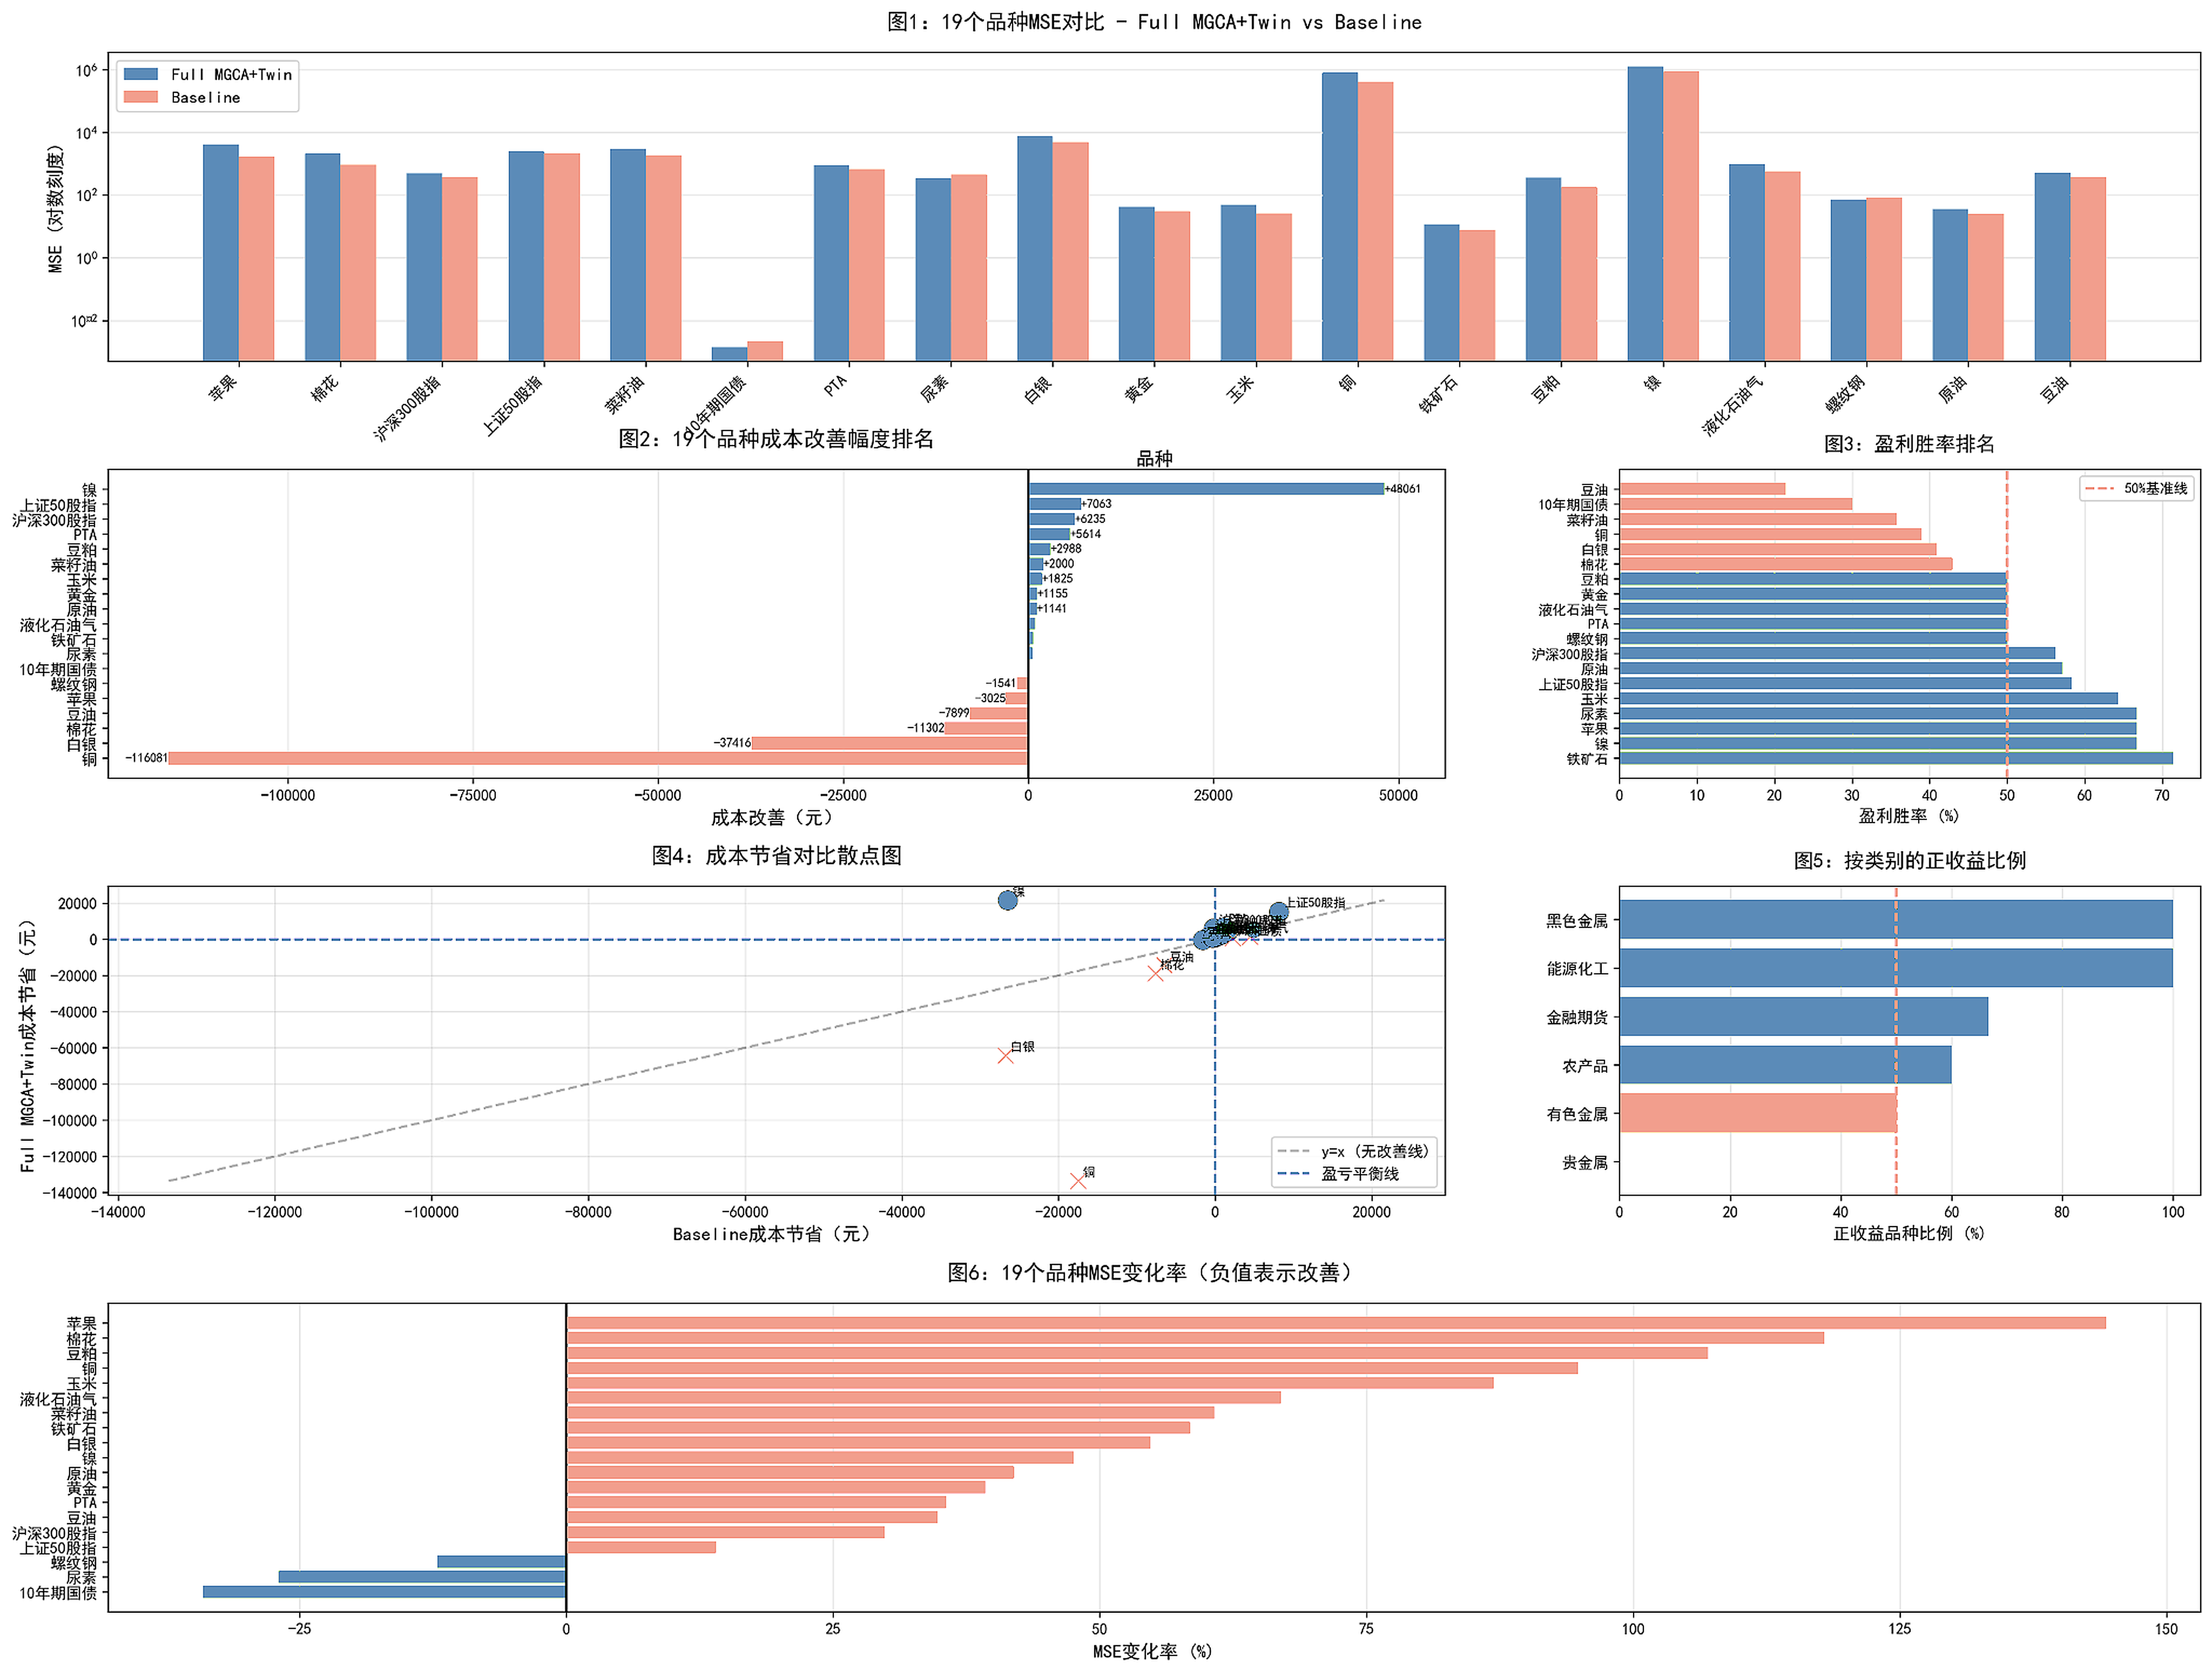
\includegraphics[width=0.95\textwidth]{figures/chap6/图5.4改.png}
\caption{孪生对抗框架在19个品种上的综合数据特征分析}
\label{fig:fullmgcatwin19varietiesdataanalysis9_new}
\end{figure}

图\ref{fig:fullmgcatwin19varietiesdataanalysis9_new}汇总了 19 个品种的均方误差分布、成本改善与盈利胜率等关键信息。结果显示，品种间预测难度与执行效果并不一致：有色金属类具有最高均方误差，但部分品种仍取得了较好的成本改善；铁矿石、镍、苹果和尿素等品种则在胜率上表现突出。这意味着，执行层优势并不简单来自拟合误差降低，而更依赖模型是否能够识别关键流动性结构并过滤异常信号。


在综合特征之外，图\ref{fig:volatilityverificationanalysis_new}进一步从波动率分层角度考察不同品种的市场状态差异。

\begin{figure}[H]
\centering
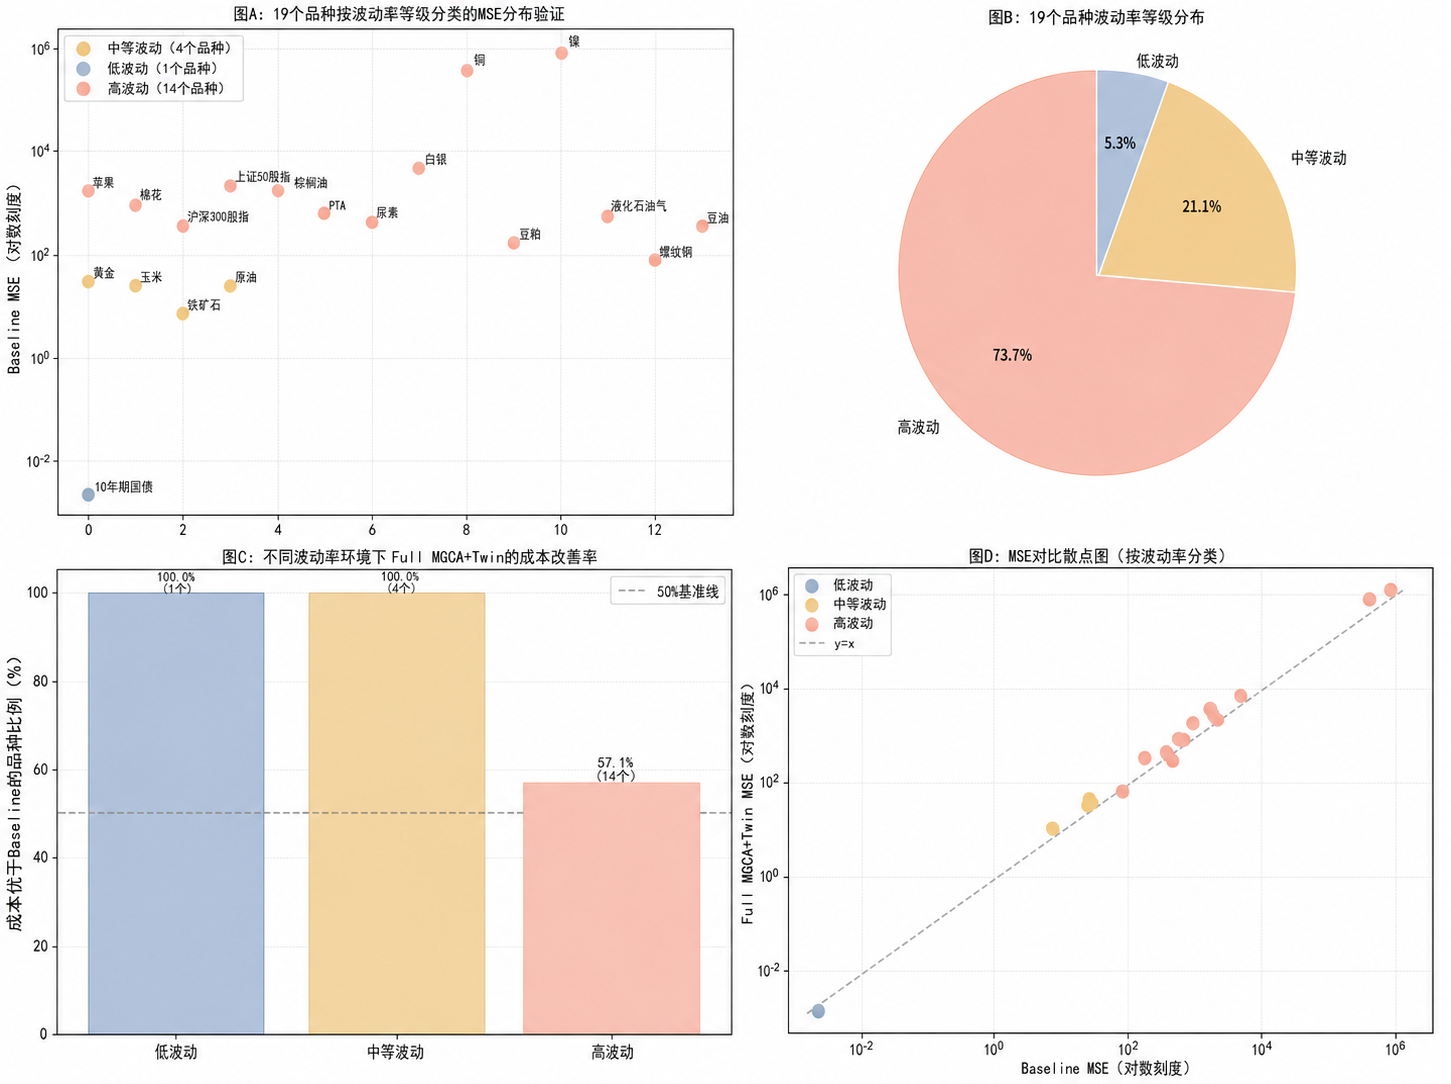
\includegraphics[width=0.85\textwidth]{figures/chap6/图5.5改}
\caption{孪生对抗框架在19个品种上的波动率分类验证与市场特征分析}
\label{fig:volatilityverificationanalysis_new}
\end{figure}

图\ref{fig:volatilityverificationanalysis_new}进一步给出了以基准模型均方误差为代理变量的波动率分层结果。低波动品种仅有 10 年期国债，中等波动品种包括铁矿石、原油、玉米和黄金，高波动品种占样本主体。在低波动和中等波动环境下，孪生对抗框架实现了 100\% 的成本改善率；即便在高波动环境中，仍有超过一半的品种获得正向改善。这表明，多生成器覆盖与孪生校验的组合，在中高波动、非平稳环境中尤其具有现实意义。

上述数据分布与波动率分层结果说明，本章实验不仅需要检验整体执行效果，还需要在不同波动状态和品种结构下考察方法的稳定性。基于此，下一节进一步说明实验设计与评价指标。

\subsection{实验设计}

本节围绕交易执行路径优化展开实验设计：在给定交易信号和执行窗口的条件下，考察不同模型如何生成下单路径，以及这些路径在滑点、成本节省和风险控制指标上的差异。实验设计包括三个层面：第一，基于高频期货数据生成成交量预测与候选执行路径；第二，将候选信号映射为 30 分钟成交量加权平均价格执行窗口内的动态下单比例；第三，通过成本节省、收益率、胜率、回撤控制和风险收益比等指标检验执行优化效果。

% 在完成候选成交量分布的生成与筛选后，调度器作为下游决策层，负责将通过认证的信号映射为可执行的下单路径\cite{bertsimas1998optimal,cartea2016closed,frei2015optimal,konishi2002optimal}。
在完成候选成交量分布的生成与筛选后，调度器作为下游决策层，负责将通过认证的信号映射为可执行的下单路径\cite{bertsimas1998optimal}。这一设置并不是将预测结果直接转化为一次性交易指令，而是先根据剩余订单量和执行时间窗口确定分段下单节奏，再检验不同模型输出能否改善成交量加权平均价格跟踪效果。最优执行问题的早期研究已从理论层面证明，在线性冲击假设下，最优策略具有封闭形式解，为后续动态调度器的设计提供了重要基础\cite{cartea2016closed}。

在随机控制框架下，Frei 与 Westray 进一步将成交量加权平均价格执行问题形式化为一类有限时间随机最优控制问题，其结论对非平稳成交量条件下的鲁棒执行具有重要参考价值\cite{frei2015optimal}。
与此同时，Konishi 从订单切片的角度出发，系统研究了如何在约束条件下实现对成交量加权平均价格基准的最优追踪，为本章调度器的分段设计提供了方法论依据\cite{konishi2002optimal}。
最优执行综述指出，现代执行模型需要在市场冲击、风险暴露、完成约束和成交量预测之间做联合权衡，而不是只优化单一成交均价\cite{gatheral2022optimal}。因此，本章实验并不只比较预测曲线是否更平滑，而是进一步检验预测结果能否形成稳定的分段下单节奏。
在日内市场中，最优下单路径会受到流动性峰谷和时间约束共同影响，静态曲线难以覆盖全部情形\cite{kath2020optimal}。这也是本文保留“预测阶段—兜底阶段”两段式安排的原因：前段依据预测成交量密度分配订单，后段在剩余时间不足或预测偏离时完成收尾。
基于长短期记忆网络的大额订单执行控制研究则表明，成交量和价格路径可以被纳入序列控制框架，为本章双阶段调度提供了方法参考\cite{papanicolaou2023optimal}。对于剩余订单量 $R_t$ 与预测成交量密度 $\hat{\mathbf{v}}=[\hat{v}_1,\dots,\hat{v}_N]$，执行器在预测阶段按照
\begin{equation}
q_t = R_t \cdot \frac{\hat{v}_t}{\sum_{k=t}^{N} \hat{v}_k}
\label{eq:dynamic_schedule_new}
\end{equation}
进行动态拆分；当进入收盘兜底阶段，则采用几何级数加速完成剩余订单：
\begin{equation}
q_t = R_t \cdot \frac{1-r}{1-r^{N-t+1}}, \qquad r\in(0,1).
\label{eq:closing_phase_new}
\end{equation}
其中，前者确保订单时间分布尽量贴近预测成交量分布，后者则在最后阶段通过加速执行保证完成率。两者结合，使得成交量加权平均价格调度既保留了对未来流动性的主动感知，又避免了因预测误差导致的未完成风险。

从执行流程看，30 分钟成交量加权平均价格窗口被划分为 30 个 1 分钟时间片。前 25 分钟属于“基于预测”阶段，执行器以未来成交量权重决定当前下单比例；后 5 分钟进入“收盘冲刺”阶段，以几何级数规则消化剩余头寸；若剩余量提前接近零，则进入“提前完成”状态。该设计将信号生成、实时分配与兜底收敛有机结合，使动态调度器能够在实际交易约束下稳定运行。成交量加权平均价格的最优执行研究表明，将成交量预测显式纳入下单路径能够提高对成交量加权平均价格基准的跟踪能力\cite{busseti2015volume}。因此，本章并不要求模型一次性给出完整订单序列，而是先预测短窗口内的成交量密度，再结合剩余订单量逐分钟更新下单比例。这样既利用了预测阶段对未来流动性的判断，也为后续兜底阶段保留了修正空间。分层深度强化学习用于成交量加权平均价格策略优化的研究也提示，执行任务可以拆成高层调度和低层执行两个子任务，从而降低单一策略直接学习完整路径的难度\cite{10336391}。

为保证后续结果可比，本章所有回测均以 10,000 单位统一下单量执行，并将每个 30 分钟窗口视作一个独立任务。每个窗口结束后，系统根据模型实现价格与基准成交量加权平均价格计算成本节省，再进一步换算为 时间段收益率、年化收益率、胜率、盈亏比、最大回撤、夏普比率、卡玛比率与索提诺比率等指标。由此，评估体系同时覆盖了拟合层指标和执行层指标，能够从拟合与执行两个层面评价策略的经济含义。

在回测框架与交易性能指标方面，本章的回测目标是量化孪生对抗框架在降低滑点、提升执行效率方面的经济价值。与单纯评价均方误差、平均绝对百分比误差的拟合分析不同，回测部分同时使用成本节省、收益率、胜率、盈亏比、最大回撤、夏普比率、卡玛比率、索提诺比率以及最大连胜连亏等指标，构成“拟合层—执行层”双重评价体系。

设每个成交量加权平均价格执行窗口的统一交易数量为 10,000 单位，投入资本定义为 $C_{\text{capital}} = Q \times \text{VWAP}_{\text{benchmark}}$。则单个窗口的收益率为
\begin{equation}
r_{\text{segment}} = \frac{\text{CostSaving}}{C_{\text{capital}}} \times 100\%.
\end{equation}
根据原始 1 分钟 K 线数据的统计结果，每日平均交易时间约为 372 分钟，对应 12.4 个 30 分钟窗口；结合每年 252 个交易日，可得年化倍数 3125。因此，年化收益率定义为 $\bar r_{\text{annual}} = \bar r_{\text{segment}} \times 3125$。其中，这里的“年化收益率”表示执行效率的年度等效表达，而不是账户复利增长。

在此框架下，成交量加权平均价格下单策略可概括为三阶段：其一，在前 25 分钟内依据预测成交量比例进行动态下单；其二，在最后 5 分钟采用几何级数规则加速完成剩余订单；其三，若剩余量已接近零，则提前停止下单。该策略与孪生校验机制结合后，使系统能够在预测和兜底之间取得平衡，避免因单一规则导致的过度交易或未完成执行。机器学习交易系统的相关思路表明，执行评价需要回到可交易规则与真实成本，而不能只依据离线预测结果判断模型优劣。

\subsection{结果分析与讨论}

本节围绕交易执行优化目标，对实验结果进行分组分析。为避免将图表简单堆叠为结果清单，下文按照“拟合表现与成交量预测—收益与胜率—风险收益结构—跨品种成本改善”的顺序展开：首先利用代表性价格预测、误差分布、训练稳定性与成交量预测结果说明候选信号是否具备进入执行路径的基础；随后结合收益率、胜率和风险收益指标，检验孪生对抗自体再生方法是否能够降低滑点传导和执行退化风险；最后通过跨品种成本改善结果讨论其适用边界。

需要说明的是，本章不以单一预测误差作为唯一评价依据，而是关注候选信号能否在真实执行窗口中转化为更稳定的下单路径。价格预测图、成交量预测图和误差分布主要用于说明模型对局部结构的刻画能力；成本节省、收益率、胜率和风险收益指标则用于检验执行路径是否在实际交易评价中降低滑点和市场冲击。

在拟合性能与成交量预测结果方面，黄金期货是本章的代表性案例之一。该数据集包含 22 个时间段，总计 55,000 个数据点，具有相对稳定但并不简单的价格结构。下文先比较价格路径拟合效果，再从误差分布、训练稳定性和成交量预测三个角度检验该机制是否能够服务于成交量加权平均价格执行优化。

首先观察价格路径拟合结果。图\ref{fig:au9999exp0baselinepredictions_new}与图\ref{fig:au9999exp7twinpredictions_new}分别给出了基准模型和孪生对抗框架在同一黄金期货时间段上的预测表现。

\begin{figure}[!htbp]
\centering
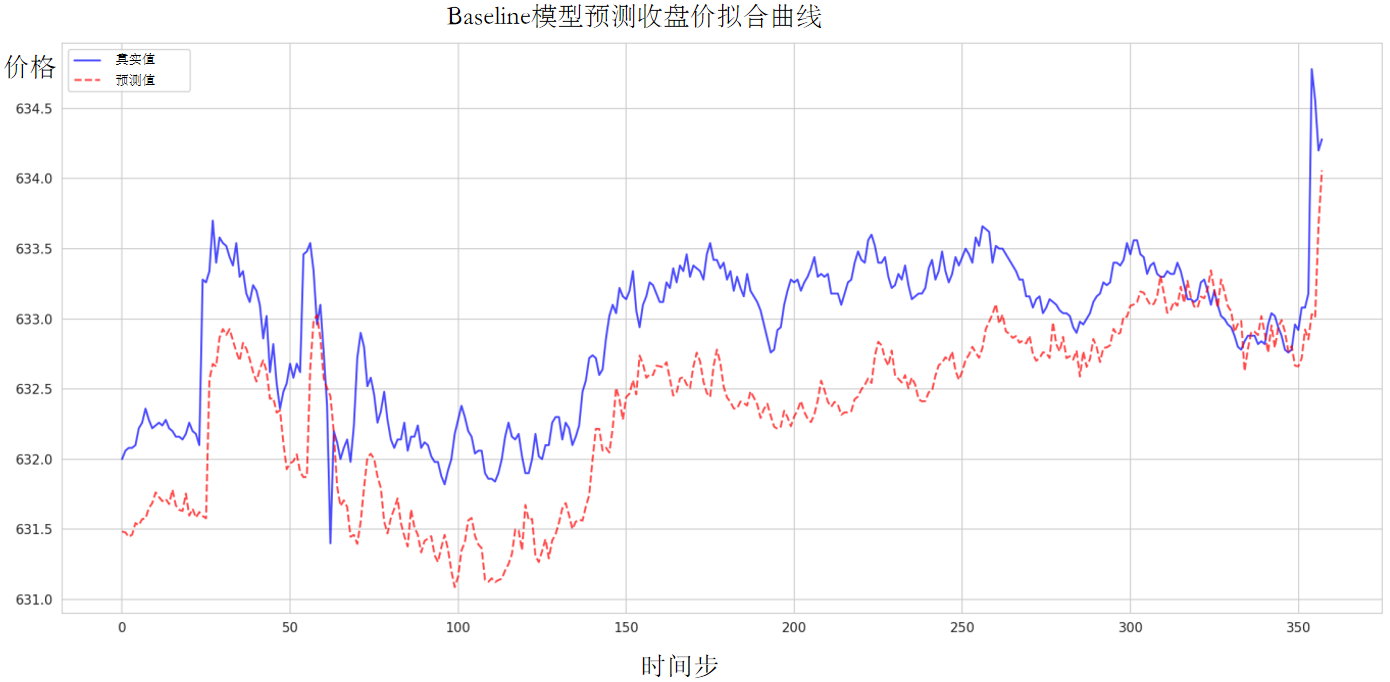
\includegraphics[width=0.80\textwidth]{figures/chap6/au_baselinepredictioncurve.png}
\caption{基准模型在黄金期货时间段002上的价格预测表现}
\label{fig:au9999exp0baselinepredictions_new}
\end{figure}

\begin{figure}[!htbp]
\centering
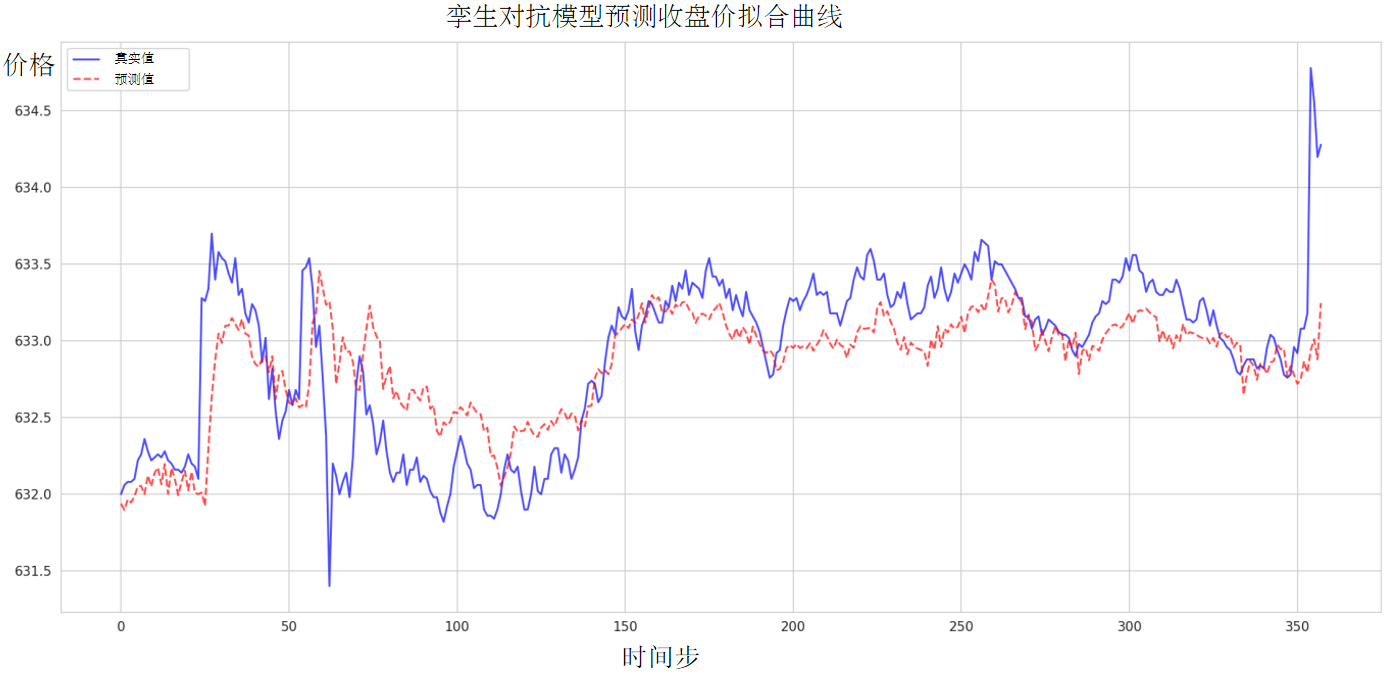
\includegraphics[width=0.80\textwidth]{figures/chap6/au_fullmgcatwinpredictioncurve.png}
\caption{孪生对抗框架在黄金期货时间段002上的价格预测表现}
\label{fig:au9999exp7twinpredictions_new}
\end{figure}

从两张价格预测图可以看出，在代表性时间段上，孪生对抗的价格预测曲线与真实价格的贴合度更高，平均绝对百分比误差由 0.0977 降至 0.0474，改善幅度为 51.51\%。这一改进并不意味着所有品种上均方误差都同步改善，但它证明了在关键局部结构上，该机制能够提供更稳定的方向捕捉能力，并在该时间段实现 2,218.80 元的成本改善。

进一步从误差分布角度观察模型稳定性。图\ref{fig:au9999exp7twinerroranaly_new}给出了孪生对抗框架在黄金期货上的误差分布结果。

\begin{figure}[!htbp]
\centering
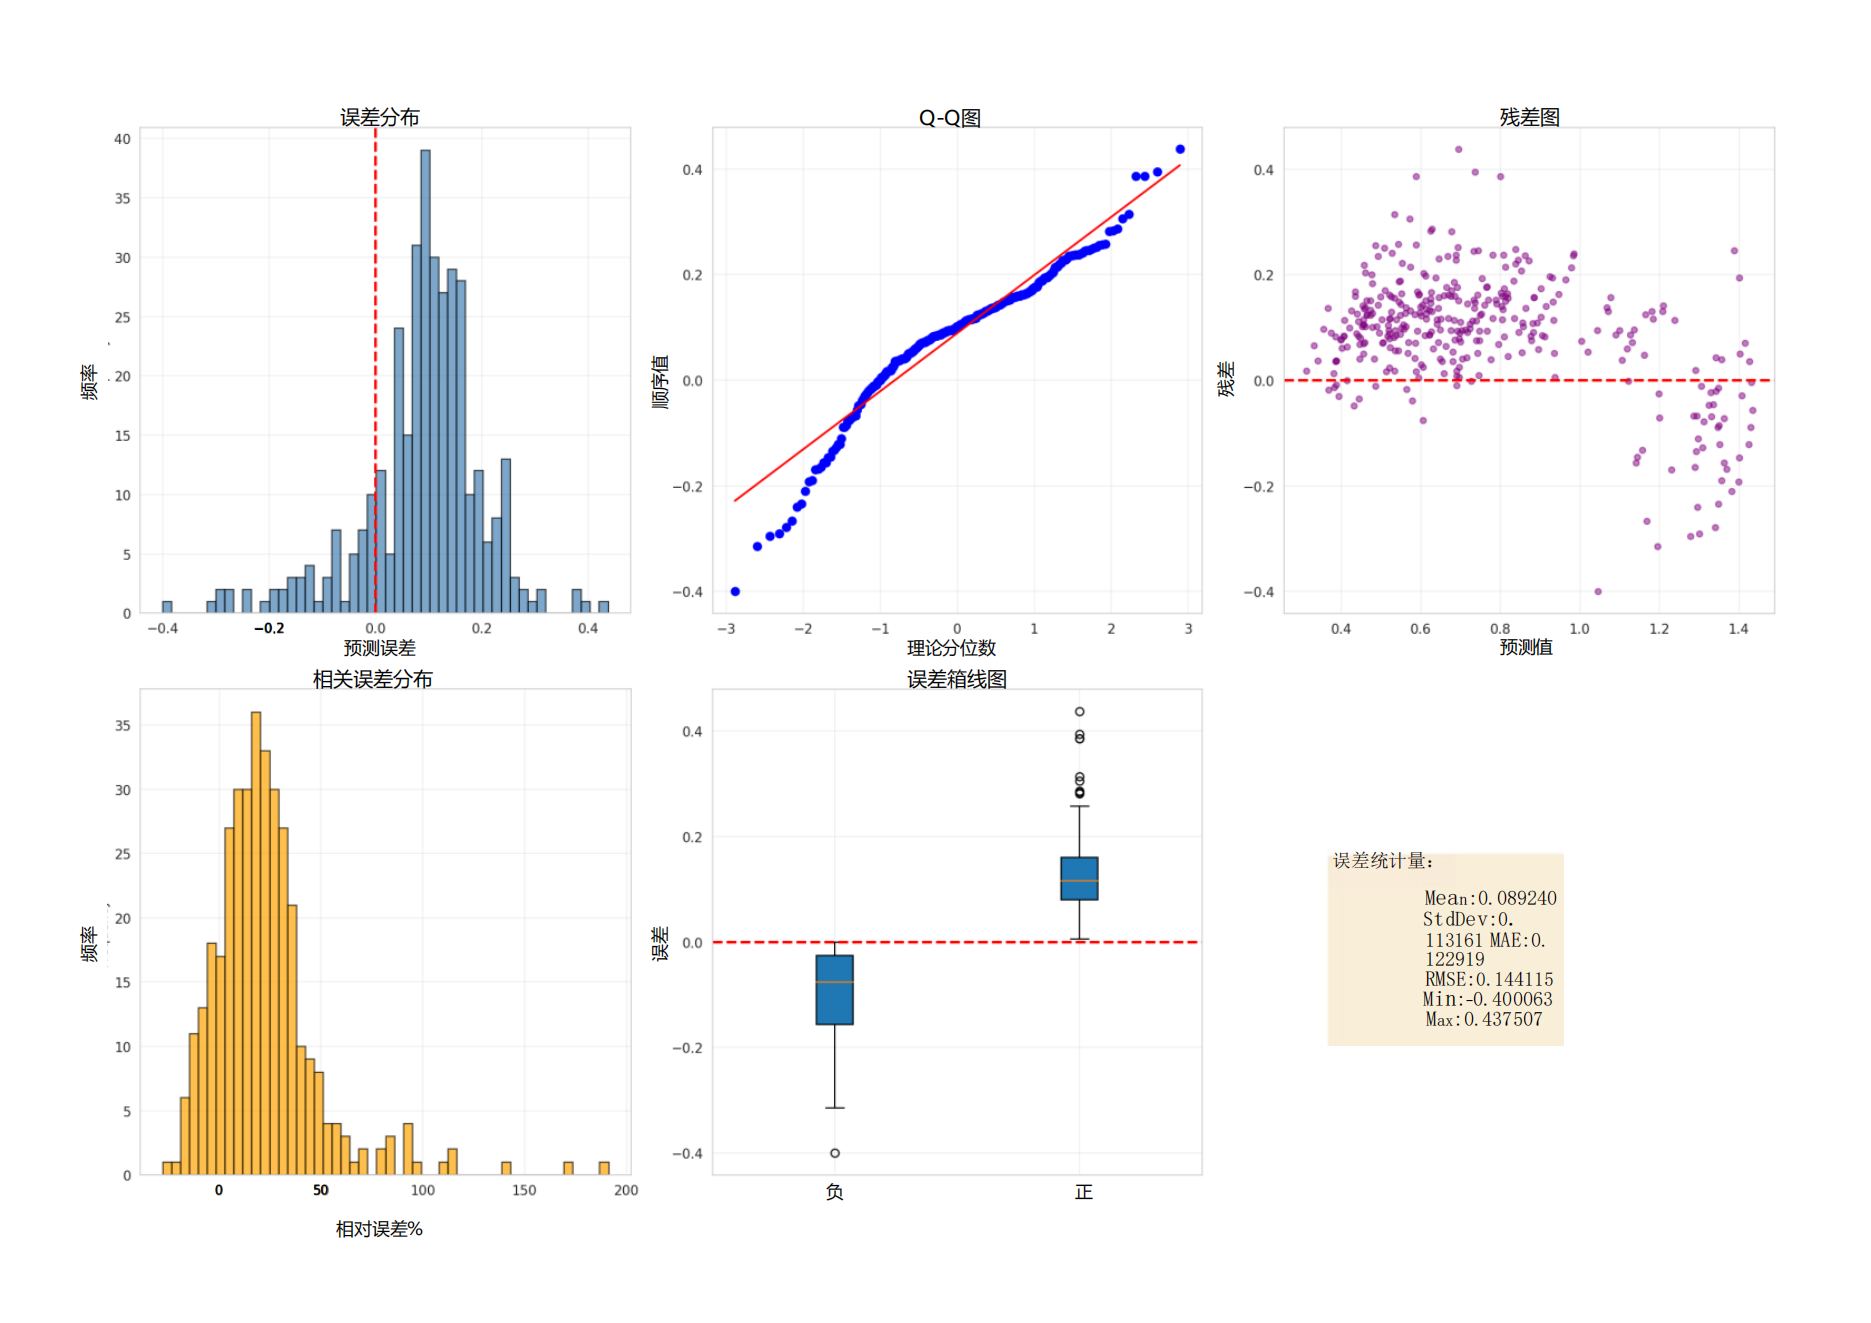
\includegraphics[width=0.80\textwidth]{figures/chap6/au_seg1_exp7_full_mgca_twin_error_analysis.png}
\caption{孪生对抗框架在黄金期货上的误差分布分析}
\label{fig:au9999exp7twinerroranaly_new}
\end{figure}

图\ref{fig:au9999exp7twinerroranaly_new}显示，黄金期货上的预测误差总体接近正态分布，残差序列未见明显结构性偏差，说明模型并非依赖单次偶然命中获得执行优势，而是在误差分布质量上具有一定稳定性。
在预测误差之外，还需要观察模型内部是否存在可用于筛选和替换的性能差异。图\ref{fig:multigencompare_new}展示了教师生成器与学生生成器在验证集上的性能分化。

\begin{figure}[!htbp]
\centering
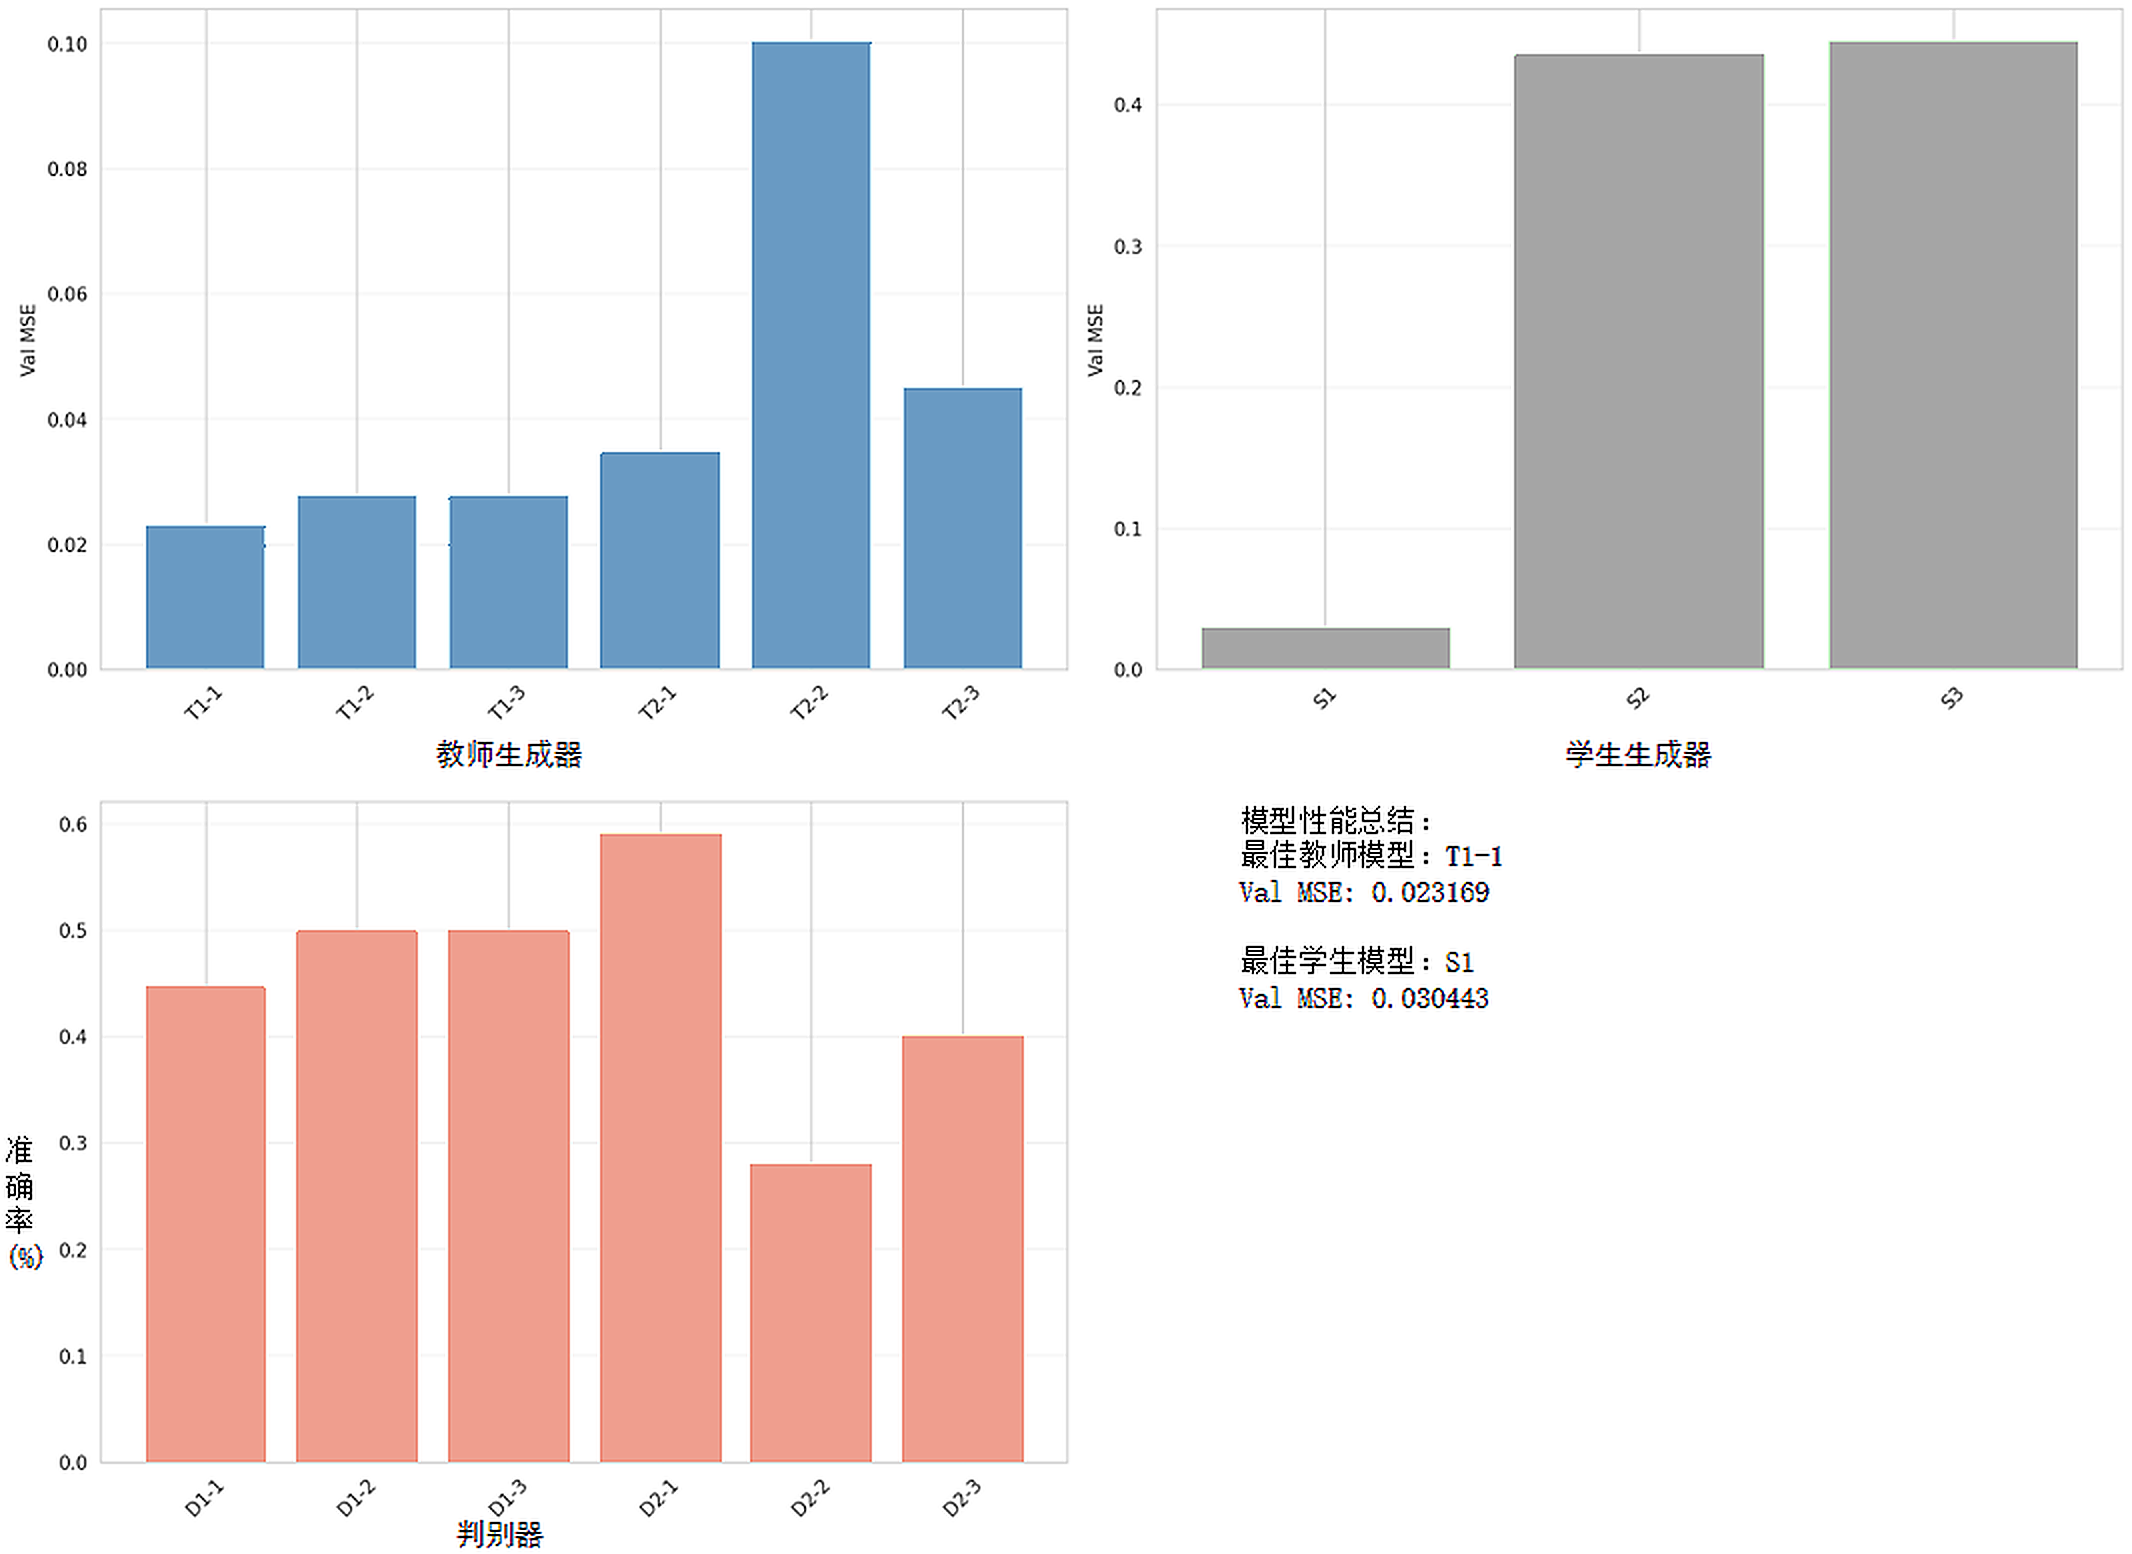
\includegraphics[width=0.80\textwidth]{figures/chap6/图5.9改.png}
\caption{孪生对抗框架在黄金期货（au数据集）上的多生成器性能对比}
\label{fig:multigencompare_new}
\end{figure}

不同成员的均方误差明显不同，这恰恰为赛马场竞争机制的动态选择和自体再生机制的偏离检测提供了基础：系统并不假定所有生成器都同样可靠，而是保留分化、比较与替换的空间。
在成员分化的基础上，图\ref{fig:au9999exp7twinvalmse_new}进一步展示了孪生对抗框架在验证集上的均方误差变化。

\begin{figure}[!htbp]
\centering
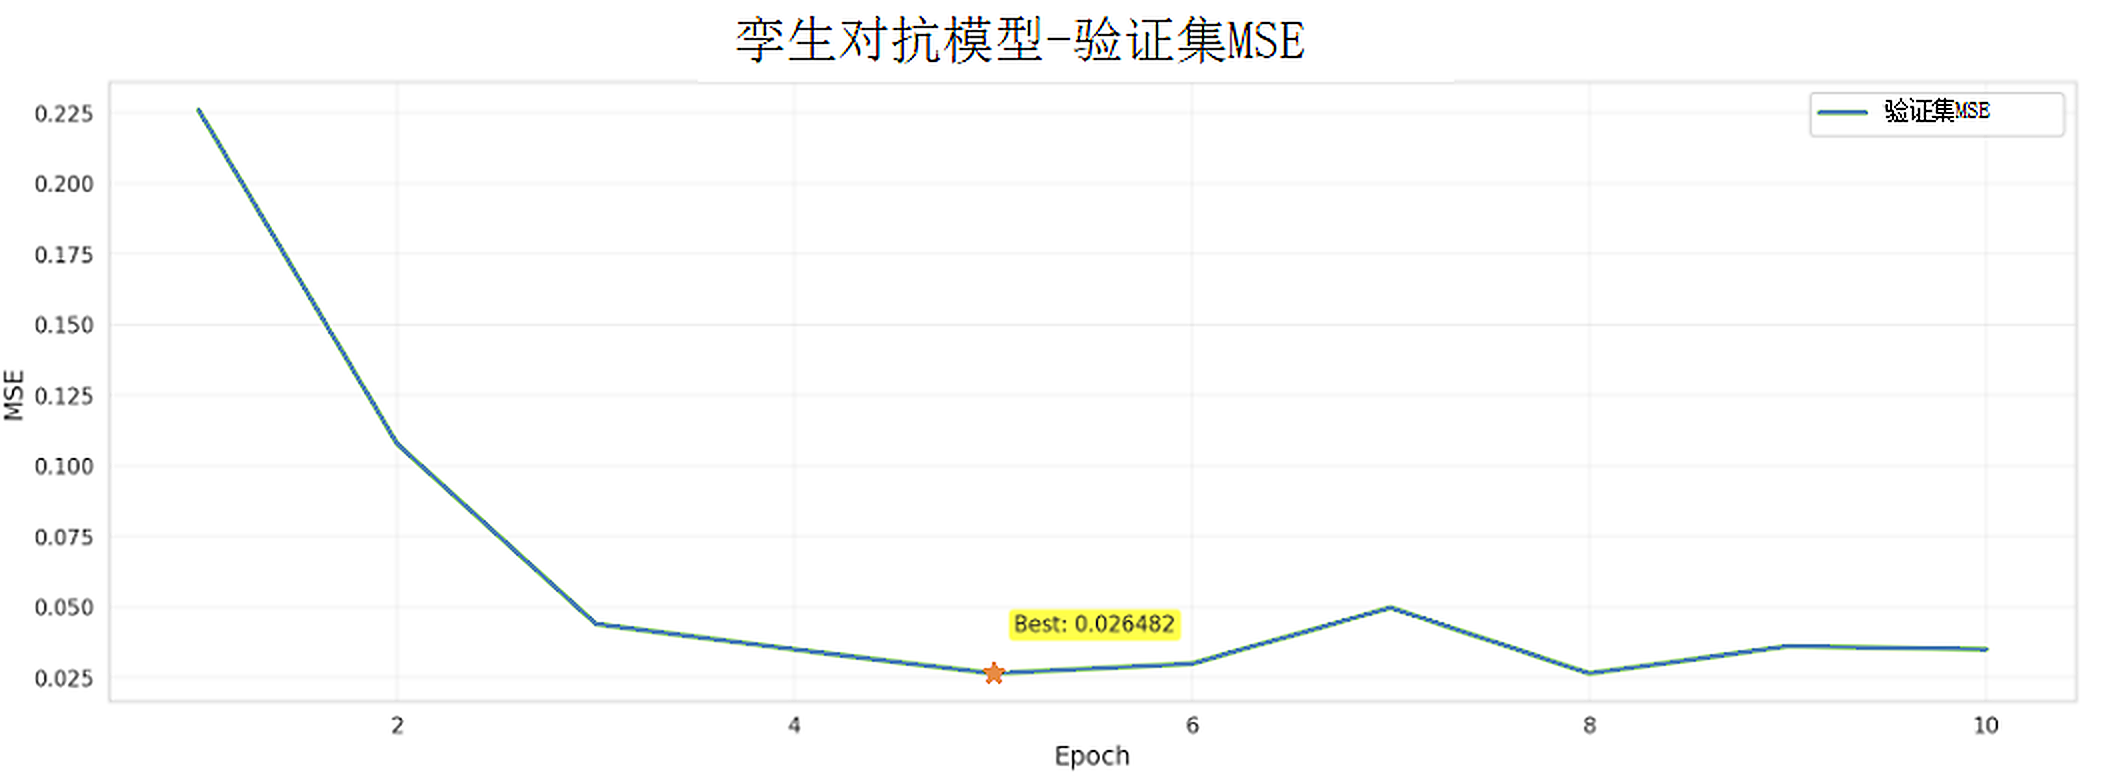
\includegraphics[width=0.80\textwidth]{figures/chap6/图5.10改.png}
\caption{孪生对抗框架在黄金期货验证集上的均方误差曲线}
\label{fig:au9999exp7twinvalmse_new}
\end{figure}

图\ref{fig:au9999exp7twinvalmse_new}表明，模型在 10 个 epoch 内较快收敛，并在第 5 个 epoch 左右达到较优泛化状态。训练过程中未出现明显崩溃，说明孪生对抗框架在该品种上表现出较好的训练稳定性。
最后转向成交量密度预测。图\ref{fig:au9999exp0baselinevolume_new}与图\ref{fig:au9999exp7twinvolume_new}分别给出基准模型和孪生对抗框架在黄金期货数据集上的成交量预测分析，用于观察模型输出能否进一步服务于订单拆分。

\begin{figure}[!htbp]
\centering
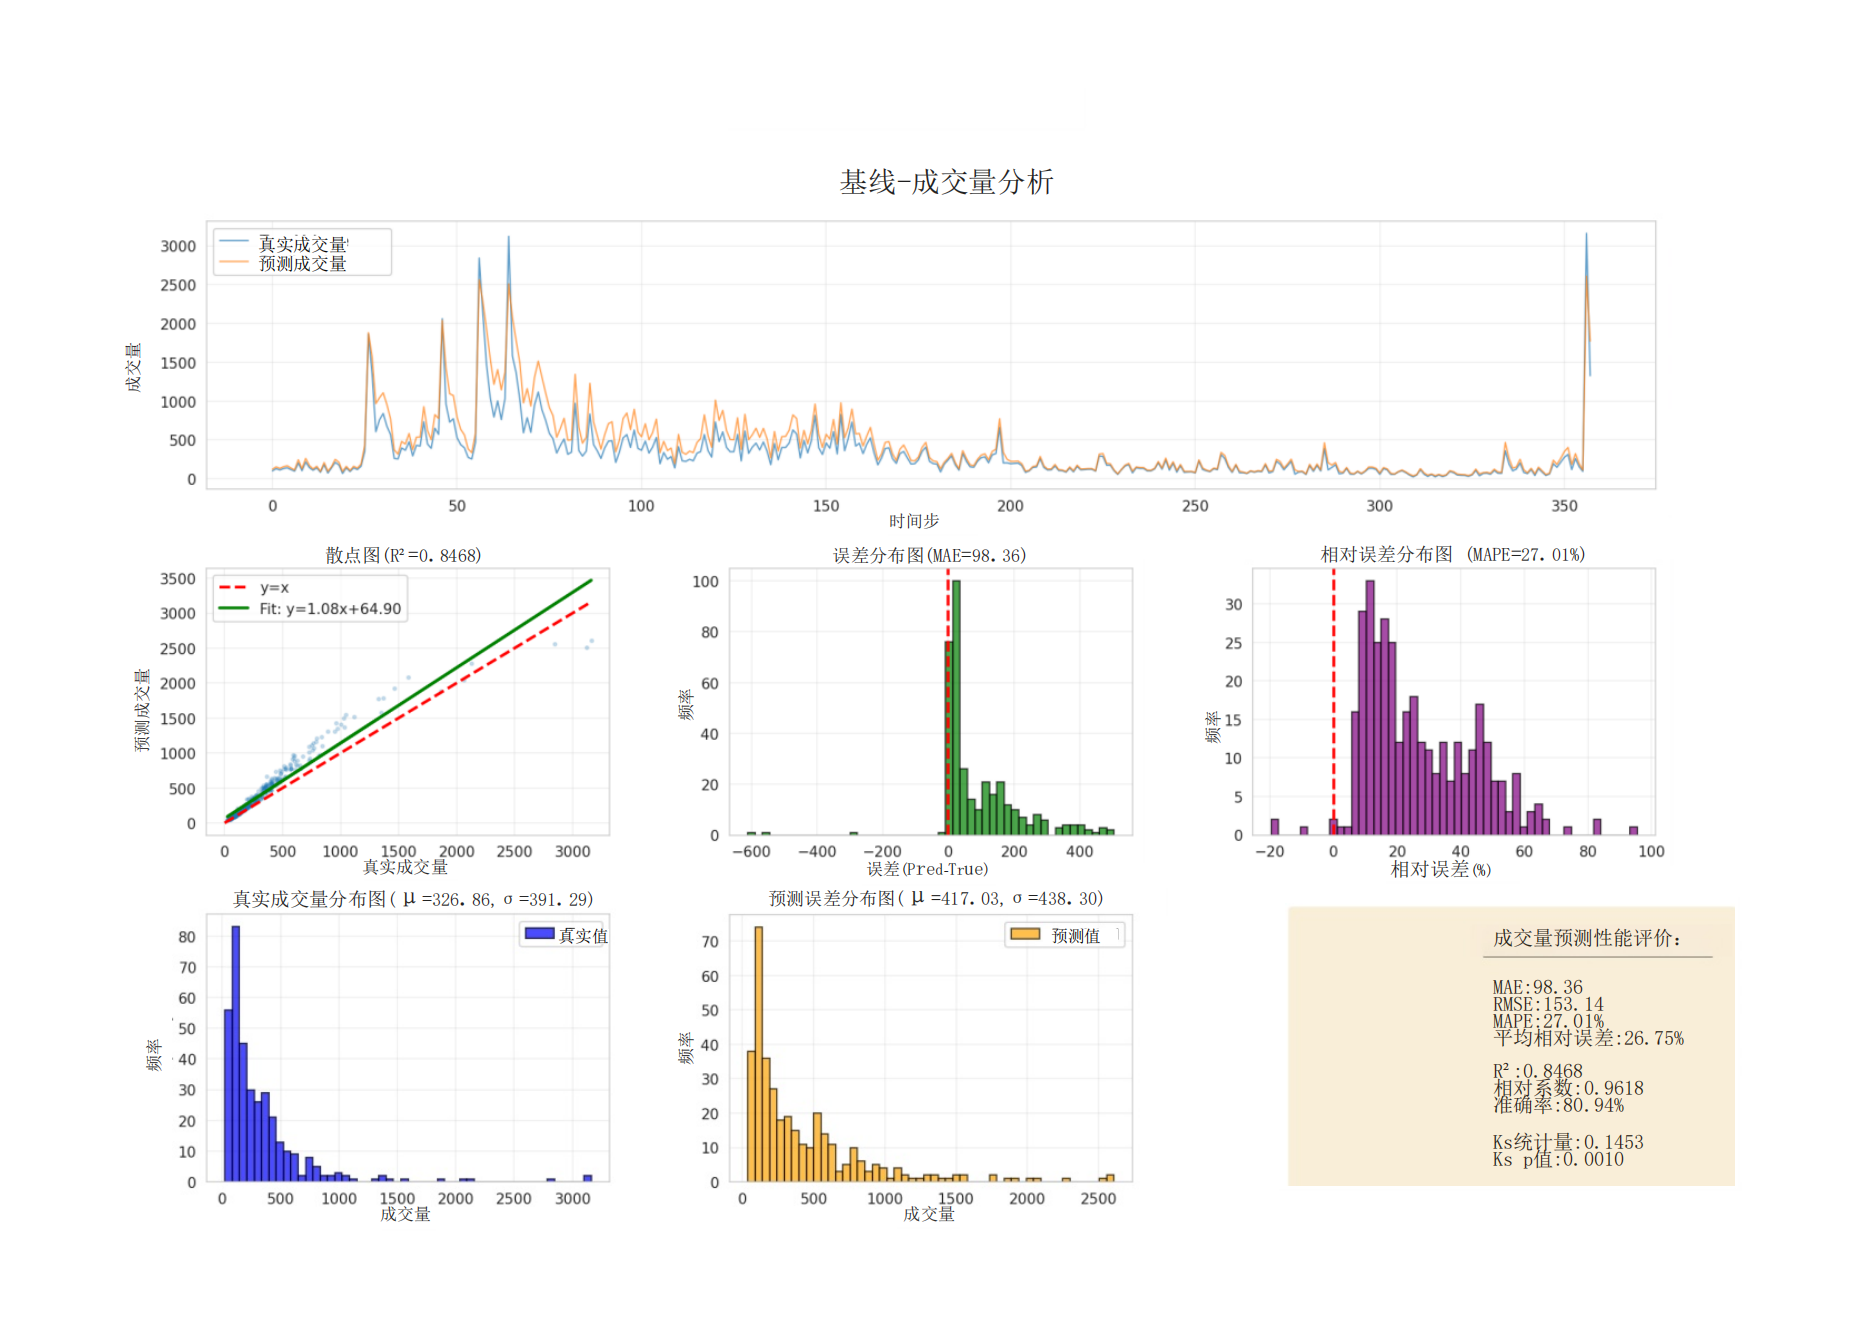
\includegraphics[width=0.80\textwidth]{figures/chap6/au_seg2_exp0_baseline_volume_analysis.png}
\caption{基准模型在黄金期货数据集上的成交量预测分析}
\label{fig:au9999exp0baselinevolume_new}
\end{figure}

\begin{figure}[!htbp]
\centering
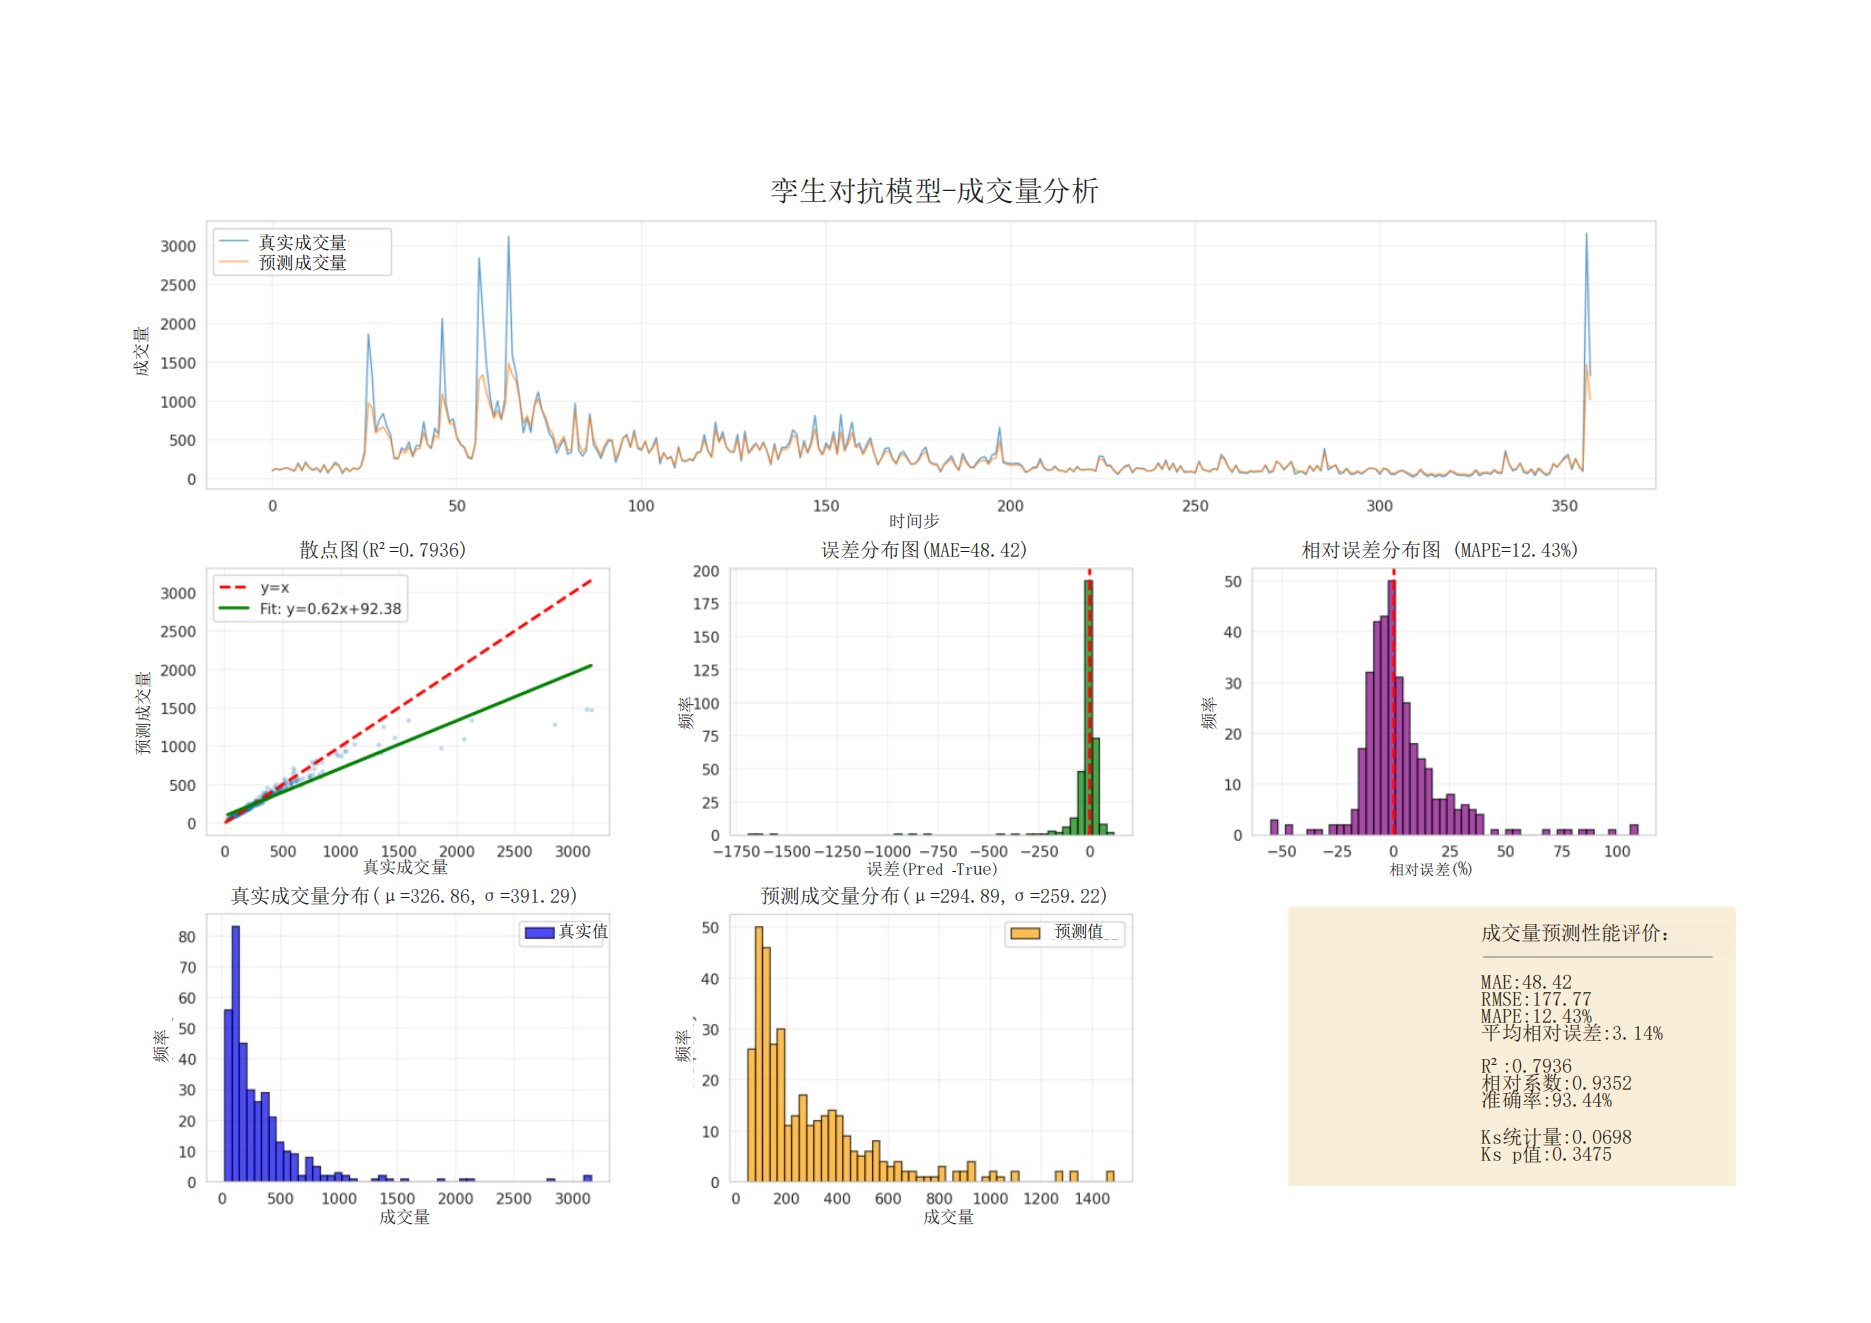
\includegraphics[width=0.80\textwidth]{figures/chap6/au_seg2_exp7_full_mgca_twin_volume_analysis.png}
\caption{孪生对抗框架在黄金期货数据集上的成交量预测分析}
\label{fig:au9999exp7twinvolume_new}
\end{figure}

图\ref{fig:au9999exp0baselinevolume_new}与图\ref{fig:au9999exp7twinvolume_new}说明，两种模型都能刻画成交量的基础趋势，但孪生对抗在峰值放量、突发缩量以及散点分布集中度上更集中。这一点对成交量加权平均价格执行较为重要，因为订单分配的好坏，本质上取决于模型是否在流动性最关键的分钟级节点上给出更可靠的成交量权重。高频市场分类中的长短期记忆网络集成研究表明，多模型结构有助于提高噪声市场中的短期方向识别能力\cite{borovkova2019ensemble}。这也解释了为什么本章不直接采用单一成交量预测器，而是通过候选生成、孪生校验和动态调度共同形成执行路径。

上述价格预测、误差分布、训练曲线和成交量预测结果共同说明，孪生对抗框架的优势并不只体现在单一预测误差下降上，更体现在局部结构识别、候选主体筛选和成交量密度刻画之间的协同。为使后续绩效表格与前述预测结果形成衔接，以下先从收益率与胜率两个直接执行指标入手，再逐步转向风险收益和连续性指标。

\FloatBarrier

% \begin{sidewaystable}
% \begin{table}
% \centering
% \footnotesize
% \setlength{\tabcolsep}{3pt}
% \begin{longtable}{lccccccccc}
% \caption{核心收益与胜率指标对比} \label{tab:twinreturnWinrate_new} \\
% \toprule


% \textbf{品种} & \textbf{时间} & \textbf{孪生对抗} & \textbf{Baseline} & \textbf{收益率} & \textbf{孪生对抗} & \textbf{Baseline} & \textbf{孪生对抗} & \textbf{Baseline} & \textbf{胜率} \\
%  & \textbf{段数} & \textbf{平均收益率} & \textbf{平均收益率} & \textbf{改善} & \textbf{年化收益率} & \textbf{年化收益率} & \textbf{胜率} & \textbf{胜率} & \textbf{提升} \\
%  & & \textbf{(\%)} & \textbf{(\%)} & \textbf{(\%)} & \textbf{(\%)} & \textbf{(\%)} & \textbf{(\%)} & \textbf{(\%)} & \textbf{(\%)} \\
% \midrule
% \endfirsthead
% \multicolumn{10}{c}{\tablename\ \thetable\ -- 续表} \\
% \toprule
% \textbf{品种} & \textbf{段数} & \textbf{孪生对抗平均} & \textbf{Baseline平均} & \textbf{收益率} & \textbf{孪生对抗年化} & \textbf{Baseline年化} & \textbf{孪生对抗} & \textbf{Baseline} & \textbf{胜率} \\
%  & & \textbf{收益率} & \textbf{收益率} & \textbf{改善} & \textbf{收益率} & \textbf{收益率} & \textbf{胜率} & \textbf{胜率} & \textbf{提升} \\
%  & & \textbf{(\%)} & \textbf{(\%)} & \textbf{(\%)} & \textbf{(\%)} & \textbf{(\%)} & \textbf{(\%)} & \textbf{(\%)} & \textbf{(\%)} \\
% \midrule
% \endhead
% \bottomrule
% \multicolumn{10}{p{0.95\textwidth}}{\footnotesize\textbf{注}：年化收益率 = 平均收益率 × 3125（年化倍数 3125 = 每日12.4个窗口 × 252交易日）。表中“年化收益率”为执行效率的年度等效百分比，非账户复利增长。}\\
% \endlastfoot
% 上证50股指 & 12 & 0.0590 & 0.0323 & 0.0267 & 184.50 & 100.96 & 58.3 & 50.0 & 8.3 \\
% 尿素 & 9 & 0.0310 & 0.0277 & 0.0034 & 97.01 & 86.45 & 66.7 & 66.7 & 0.0 \\
% 原油 & 21 & 0.0174 & -0.0058 & 0.0232 & 54.53 & -18.02 & 57.1 & 33.3 & 23.8 \\
% 沪深300股指 & 16 & 0.0162 & -0.0001 & 0.0163 & 50.59 & -0.46 & 56.2 & 43.8 & 12.5 \\
% 豆粕 & 14 & 0.0150 & 0.0056 & 0.0094 & 46.93 & 17.41 & 50.0 & 57.1 & -7.1 \\
% PTA & 14 & 0.0140 & 0.0023 & 0.0118 & 43.89 & 7.10 & 50.0 & 42.9 & 7.1 \\
% 铁矿石 & 14 & 0.0138 & 0.0058 & 0.0080 & 43.12 & 18.11 & 71.4 & 50.0 & 21.4 \\
% 玉米 & 14 & 0.0115 & 0.0034 & 0.0081 & 36.02 & 10.69 & 64.3 & 50.0 & 14.3 \\
% 液化石油气 & 14 & 0.0032 & 0.0018 & 0.0014 & 9.98 & 5.68 & 50.0 & 64.3 & -14.3 \\
% 苹果 & 9 & 0.0026 & 0.0057 & -0.0032 & 8.02 & 17.95 & 66.7 & 66.7 & 0.0 \\
% 镍 & 18 & 0.0018 & -0.0021 & 0.0039 & 5.50 & -6.60 & 66.7 & 44.4 & 22.2 \\
% 螺纹钢 & 14 & 0.0017 & 0.0071 & -0.0054 & 5.32 & 22.09 & 50.0 & 71.4 & -21.4 \\
% 菜籽油 & 14 & 0.0001 & -0.0013 & 0.0014 & 0.43 & -3.93 & 35.7 & 28.6 & 7.1 \\
% 10年期国债 & 10 & -0.0008 & -0.0008 & 0.0000 & -2.39 & -2.46 & 30.0 & 40.0 & -10.0 \\
% 黄金 & 22 & -0.0069 & -0.0245 & 0.0176 & -21.61 & -76.54 & 50.0 & 40.9 & 9.1 \\
% 棉花 & 14 & -0.0142 & -0.0057 & -0.0084 & -44.30 & -17.90 & 42.9 & 35.7 & 7.1 \\
% 铜 & 18 & -0.0175 & -0.0023 & -0.0151 & -54.65 & -7.33 & 38.9 & 50.0 & -11.1 \\
% 豆油 & 14 & -0.0183 & -0.0082 & -0.0101 & -57.25 & -25.74 & 21.4 & 28.6 & -7.1 \\
% 白银 & 22 & -0.0823 & -0.0344 & -0.0480 & -257.29 & -107.42 & 40.9 & 50.0 & -9.1 \\
% \end{longtable}
% % \end{sidewaystable}
% \end{table}
\begin{table}[!htbp]
\centering
\caption{核心收益与胜率指标对比}
\label{tab:core_compare}
\footnotesize
\setlength{\tabcolsep}{2pt}
\renewcommand{\arraystretch}{1.18}
\begin{tabular}{@{}p{0.12\textwidth}p{0.055\textwidth}p{0.13\textwidth}p{0.13\textwidth}p{0.105\textwidth}p{0.13\textwidth}p{0.13\textwidth}@{}}
\toprule
\textbf{品种} &
\makecell{\textbf{时间}\\\textbf{段数}} &
\makecell{\textbf{孪生对抗}\\\textbf{平均}\\\textbf{收益率(\%)}} &
\makecell{\textbf{基准模型}\\\textbf{平均}\\\textbf{收益率(\%)}} &
\makecell{\textbf{收益率}\\\textbf{改善(\%)}} &
\makecell{\textbf{孪生对抗}\\\textbf{年化}\\\textbf{收益率(\%)}} &
\makecell{\textbf{基准模型}\\\textbf{年化}\\\textbf{收益率(\%)}} \\
\midrule
上证50股指 & 12 & 0.0590 & 0.0323 & 0.0267 & 184.50 & 100.96 \\
尿素 & 9 & 0.0310 & 0.0277 & 0.0034 & 97.01 & 86.45 \\
原油 & 21 & 0.0174 & -0.0058 & 0.0232 & 54.53 & -18.02 \\
沪深300股指 & 16 & 0.0162 & -0.0001 & 0.0163 & 50.59 & -0.46 \\
豆粕 & 14 & 0.0150 & 0.0056 & 0.0094 & 46.93 & 17.41 \\
PTA & 14 & 0.0140 & 0.0023 & 0.0118 & 43.89 & 7.10 \\
铁矿石 & 14 & 0.0138 & 0.0058 & 0.0080 & 43.12 & 18.11 \\
玉米 & 14 & 0.0115 & 0.0034 & 0.0081 & 36.02 & 10.69 \\
液化石油气 & 14 & 0.0032 & 0.0018 & 0.0014 & 9.98 & 5.68 \\
苹果 & 9 & 0.0026 & 0.0057 & -0.0032 & 8.02 & 17.95 \\
镍 & 18 & 0.0018 & -0.0021 & 0.0039 & 5.50 & -6.60 \\
螺纹钢 & 14 & 0.0017 & 0.0071 & -0.0054 & 5.32 & 22.09 \\
菜籽油 & 14 & 0.0001 & -0.0013 & 0.0014 & 0.43 & -3.93 \\
10年期国债 & 10 & -0.0008 & -0.0008 & 0.0000 & -2.39 & -2.46 \\
黄金 & 22 & -0.0069 & -0.0245 & 0.0176 & -21.61 & -76.54 \\
棉花 & 14 & -0.0142 & -0.0057 & -0.0084 & -44.30 & -17.90 \\
铜 & 18 & -0.0175 & -0.0023 & -0.0151 & -54.65 & -7.33 \\
豆油 & 14 & -0.0183 & -0.0082 & -0.0101 & -57.25 & -25.74 \\
白银 & 22 & -0.0823 & -0.0344 & -0.0480 & -257.29 & -107.42 \\
\bottomrule
\end{tabular}
\end{table}
\begin{table}[!htbp]
\centering
{\small\textbf{续表}}\\[0.5em]
\footnotesize
\setlength{\tabcolsep}{3pt}
\renewcommand{\arraystretch}{1.18}
\begin{tabular}{@{}p{0.16\textwidth}p{0.18\textwidth}p{0.18\textwidth}p{0.18\textwidth}p{0.14\textwidth}@{}}
\toprule
\textbf{品种} & \textbf{时间段数} & \makecell{\textbf{孪生对抗}\\\textbf{胜率(\%)}} & \makecell{\textbf{基准模型}\\\textbf{胜率(\%)}} & \makecell{\textbf{胜率}\\\textbf{提升(\%)}} \\
\midrule
上证50股指 & 12 & 58.3 & 50.0 & 8.3 \\
尿素 & 9 & 66.7 & 66.7 & 0.0 \\
原油 & 21 & 57.1 & 33.3 & 23.8 \\
沪深300股指 & 16 & 56.2 & 43.8 & 12.5 \\
豆粕 & 14 & 50.0 & 57.1 & -7.1 \\
PTA & 14 & 50.0 & 42.9 & 7.1 \\
铁矿石 & 14 & 71.4 & 50.0 & 21.4 \\
玉米 & 14 & 64.3 & 50.0 & 14.3 \\
液化石油气 & 14 & 50.0 & 64.3 & -14.3 \\
苹果 & 9 & 66.7 & 66.7 & 0.0 \\
镍 & 18 & 66.7 & 44.4 & 22.2 \\
螺纹钢 & 14 & 50.0 & 71.4 & -21.4 \\
菜籽油 & 14 & 35.7 & 28.6 & 7.1 \\
10年期国债 & 10 & 30.0 & 40.0 & -10.0 \\
黄金 & 22 & 50.0 & 40.9 & 9.1 \\
棉花 & 14 & 42.9 & 35.7 & 7.1 \\
铜 & 18 & 38.9 & 50.0 & -11.1 \\
豆油 & 14 & 21.4 & 28.6 & -7.1 \\
白银 & 22 & 40.9 & 50.0 & -9.1 \\
\bottomrule
\end{tabular}
\end{table}

表\ref{tab:core_compare}给出了收益率与胜率的对比结果。总体上，19 个品种中有 12 个在平均收益率维度获得改善，上证50股指、原油、沪深300股指、PTA 和铁矿石等品种表现尤为突出。其中，上证50股指的每 30 分钟平均收益率达到 0.0590\%，对应年化等效 184.50\%；原油和沪深300股指则实现了从基准模型负收益到该机制正收益的转变。相较之下，白银、铜和豆油等高噪声品种仍然表现较弱，提示机制存在明确的适用边界。

在收益率与胜率之外，还需要进一步观察收益是否伴随过高回撤或下行波动。如果执行优化只提升局部收益而同步放大尾部风险，则难以作为稳定执行模块嵌入真实交易系统。因此，表\ref{tab:twinriskReturn_new}进一步给出盈亏比、最大回撤、夏普比率与卡玛比率等风险收益指标。

\FloatBarrier

% \begin{sidewaystable}
\begin{table}[!htbp]
\centering
\caption{风险收益比指标对比}
\label{tab:twinriskReturn_new}
\small
\setlength{\tabcolsep}{6pt}
\renewcommand{\arraystretch}{1.18}
\begin{tabular}{lcccc}
\toprule
\textbf{品种} & \makecell{\textbf{孪生对抗}\\\textbf{盈亏比}} & \makecell{\textbf{基准模型}\\\textbf{盈亏比}} & \makecell{\textbf{孪生对抗}\\\textbf{最大回撤(\%)}} & \makecell{\textbf{基准模型}\\\textbf{最大回撤(\%)}} \\
\midrule
上证50股指 & 10.57 & 6.65 & 41.17 & 100.00 \\
尿素 & 1.30 & 4.85 & 42.12 & 15.07 \\
原油 & 2.01 & 1.15 & 100.00 & 88.03 \\
沪深300股指 & 1.93 & 1.27 & 90.82 & 100.00 \\
豆粕 & 2.35 & 1.49 & 100.00 & 100.00 \\
PTA & 1.95 & 1.69 & 91.69 & 84.17 \\
铁矿石 & 0.66 & 1.83 & 82.61 & 86.51 \\
玉米 & 1.31 & 1.91 & 28.39 & 60.25 \\
液化石油气 & 1.23 & 0.78 & 100.00 & 100.00 \\
苹果 & 0.58 & 0.86 & 100.00 & 100.00 \\
镍 & 0.60 & 0.94 & 86.25 & 100.00 \\
螺纹钢 & 1.17 & 1.27 & 77.61 & 59.32 \\
菜籽油 & 1.81 & 2.17 & 97.10 & 100.00 \\
10年期国债 & 1.37 & 0.88 & 100.00 & 100.00 \\
黄金 & 0.63 & 0.18 & 100.00 & 100.00 \\
棉花 & 0.43 & 0.55 & 100.00 & 100.00 \\
铜 & 0.34 & 0.56 & 87.95 & 83.11 \\
豆油 & 0.34 & 1.31 & 100.00 & 100.00 \\
白银 & 0.14 & 0.16 & 100.00 & 100.00 \\
\bottomrule
\end{tabular}
\end{table}
\begin{table}[!htbp]
\centering
{\small\textbf{续表}}\\[0.5em]
\small
\setlength{\tabcolsep}{7pt}
\renewcommand{\arraystretch}{1.18}
\begin{tabular}{lcccc}
\toprule
\textbf{品种} & \makecell{\textbf{孪生对抗}\\\textbf{夏普比率}} & \makecell{\textbf{基准模型}\\\textbf{夏普比率}} & \makecell{\textbf{孪生对抗}\\\textbf{卡玛比率}} & \makecell{\textbf{基准模型}\\\textbf{卡玛比率}} \\
\midrule
上证50股指 & 31.05 & 18.03 & 4.48 & 1.01 \\
尿素 & 15.40 & 39.88 & 2.30 & 5.74 \\
原油 & 14.64 & -11.32 & 0.55 & -0.20 \\
沪深300股指 & 18.51 & -0.23 & 0.56 & -0.00 \\
豆粕 & 14.75 & 13.43 & 0.47 & 0.17 \\
PTA & 12.12 & 4.75 & 0.48 & 0.08 \\
铁矿石 & 9.12 & 11.61 & 0.52 & 0.21 \\
玉米 & 18.15 & 14.64 & 1.27 & 0.18 \\
液化石油气 & 3.32 & 7.24 & 0.10 & 0.06 \\
苹果 & 3.01 & 9.59 & 0.08 & 0.18 \\
镍 & 3.66 & -5.76 & 0.06 & -0.07 \\
螺纹钢 & 3.07 & 22.41 & 0.07 & 0.37 \\
菜籽油 & 0.10 & -2.55 & 0.00 & -0.04 \\
10年期国债 & -10.77 & -12.05 & -0.02 & -0.02 \\
黄金 & -8.03 & -16.03 & -0.22 & -0.77 \\
棉花 & -19.82 & -22.28 & -0.44 & -0.18 \\
铜 & -21.69 & -12.01 & -0.62 & -0.09 \\
豆油 & -36.70 & -10.80 & -0.57 & -0.26 \\
白银 & -15.09 & -13.64 & -2.57 & -1.07 \\
\bottomrule
\end{tabular}
\end{table}

表\ref{tab:twinriskReturn_new}揭示了更细粒度的风险收益结构。上证50股指在盈亏比、夏普比率和卡玛比率三个维度上同时领先，说明其高收益并非来自偶然命中，而是建立在较优风险控制基础之上；玉米的最大回撤仅为 28.39\%，在风险控制维度表现突出；原油与沪深300股指则实现了夏普比率由负转正。与此同时，若干品种的最大回撤仍达到 100\%，说明在极端高噪声条件下，孪生对抗虽能改善执行效率，但尚不能完全消除尾部风险。
风险收益指标反映的是整体分布特征，尚不能完全说明盈利或亏损在时间序列中的连续性。为进一步判断执行路径是否容易出现连续失效，表\ref{tab:twinadvancedMetrics_new}从下行风险和连胜连亏角度补充检验。

\FloatBarrier

% \begin{sidewaystable}
\begin{table}[!htbp]
\centering
\caption{高级绩效指标对比}
\label{tab:twinadvancedMetrics_new}
\small
\setlength{\tabcolsep}{5pt}
\renewcommand{\arraystretch}{1.18}
\begin{tabular}{lcccccc}
\toprule
\textbf{品种} & \makecell{\textbf{孪生对抗}\\\textbf{索提诺比率}} & \makecell{\textbf{基准模型}\\\textbf{索提诺比率}} & \makecell{\textbf{孪生对抗}\\\textbf{最大连胜}} & \makecell{\textbf{孪生对抗}\\\textbf{最大连亏}} & \makecell{\textbf{基准模型}\\\textbf{最大连胜}} & \makecell{\textbf{基准模型}\\\textbf{最大连亏}} \\
\midrule
上证50股指 & 319.21 & 117.17 & 3 & 2 & 3 & 4 \\
尿素 & 44.22 & 162.03 & 3 & 2 & 4 & 2 \\
原油 & 38.82 & -15.98 & 3 & 3 & 3 & 6 \\
沪深300股指 & 33.80 & -0.36 & 3 & 3 & 3 & 5 \\
豆粕 & 30.78 & 32.47 & 5 & 5 & 3 & 2 \\
PTA & 29.26 & 6.97 & 4 & 3 & 2 & 3 \\
铁矿石 & 8.87 & 17.54 & 5 & 2 & 4 & 3 \\
玉米 & 30.91 & 29.88 & 3 & 2 & 2 & 2 \\
液化石油气 & 3.79 & 10.11 & 4 & 3 & 5 & 3 \\
苹果 & 3.79 & 16.65 & 2 & 1 & 2 & 1 \\
\bottomrule
\end{tabular}
\end{table}
\begin{table}[!htbp]
\centering
{\small\textbf{续表}}\\[0.5em]
\small
\setlength{\tabcolsep}{5pt}
\renewcommand{\arraystretch}{1.18}
\begin{tabular}{lcccccc}
\toprule
\textbf{品种} & \makecell{\textbf{孪生对抗}\\\textbf{索提诺比率}} & \makecell{\textbf{基准模型}\\\textbf{索提诺比率}} & \makecell{\textbf{孪生对抗}\\\textbf{最大连胜}} & \makecell{\textbf{孪生对抗}\\\textbf{最大连亏}} & \makecell{\textbf{基准模型}\\\textbf{最大连胜}} & \makecell{\textbf{基准模型}\\\textbf{最大连亏}} \\
\midrule
镍 & 6.76 & -10.70 & 4 & 3 & 3 & 3 \\
螺纹钢 & 4.41 & 35.42 & 3 & 2 & 5 & 2 \\
菜籽油 & 0.21 & -7.93 & 2 & 4 & 1 & 5 \\
10年期国债 & -25.40 & -33.62 & 2 & 3 & 2 & 3 \\
黄金 & -8.72 & -12.86 & 3 & 6 & 4 & 5 \\
棉花 & -21.85 & -25.95 & 3 & 4 & 2 & 4 \\
铜 & -20.34 & -14.53 & 3 & 4 & 4 & 4 \\
豆油 & -38.31 & -20.77 & 2 & 7 & 1 & 5 \\
白银 & -11.95 & -10.05 & 3 & 4 & 4 & 5 \\
\bottomrule
\end{tabular}
\end{table}

表\ref{tab:twinadvancedMetrics_new}从下行风险与连续性维度补充了执行表现。上证50股指、原油、沪深300股指、豆粕、PTA 与玉米的索提诺比率较高，说明这些品种在控制下行波动方面优于整体波动表现；豆粕和铁矿石的最大连胜均达到 5，体现出盈利持续性；豆油的最大连亏为 7，则反映了高噪声品种在连续亏损压力上的约束。

在分别完成收益、风险与连续性指标分析后，图\ref{fig:comprehensiveviz_new}将上述评价维度集中呈现，用于辅助观察不同品种在多指标空间中的相对位置。

\FloatBarrier

\begin{figure}[!p]
\centering
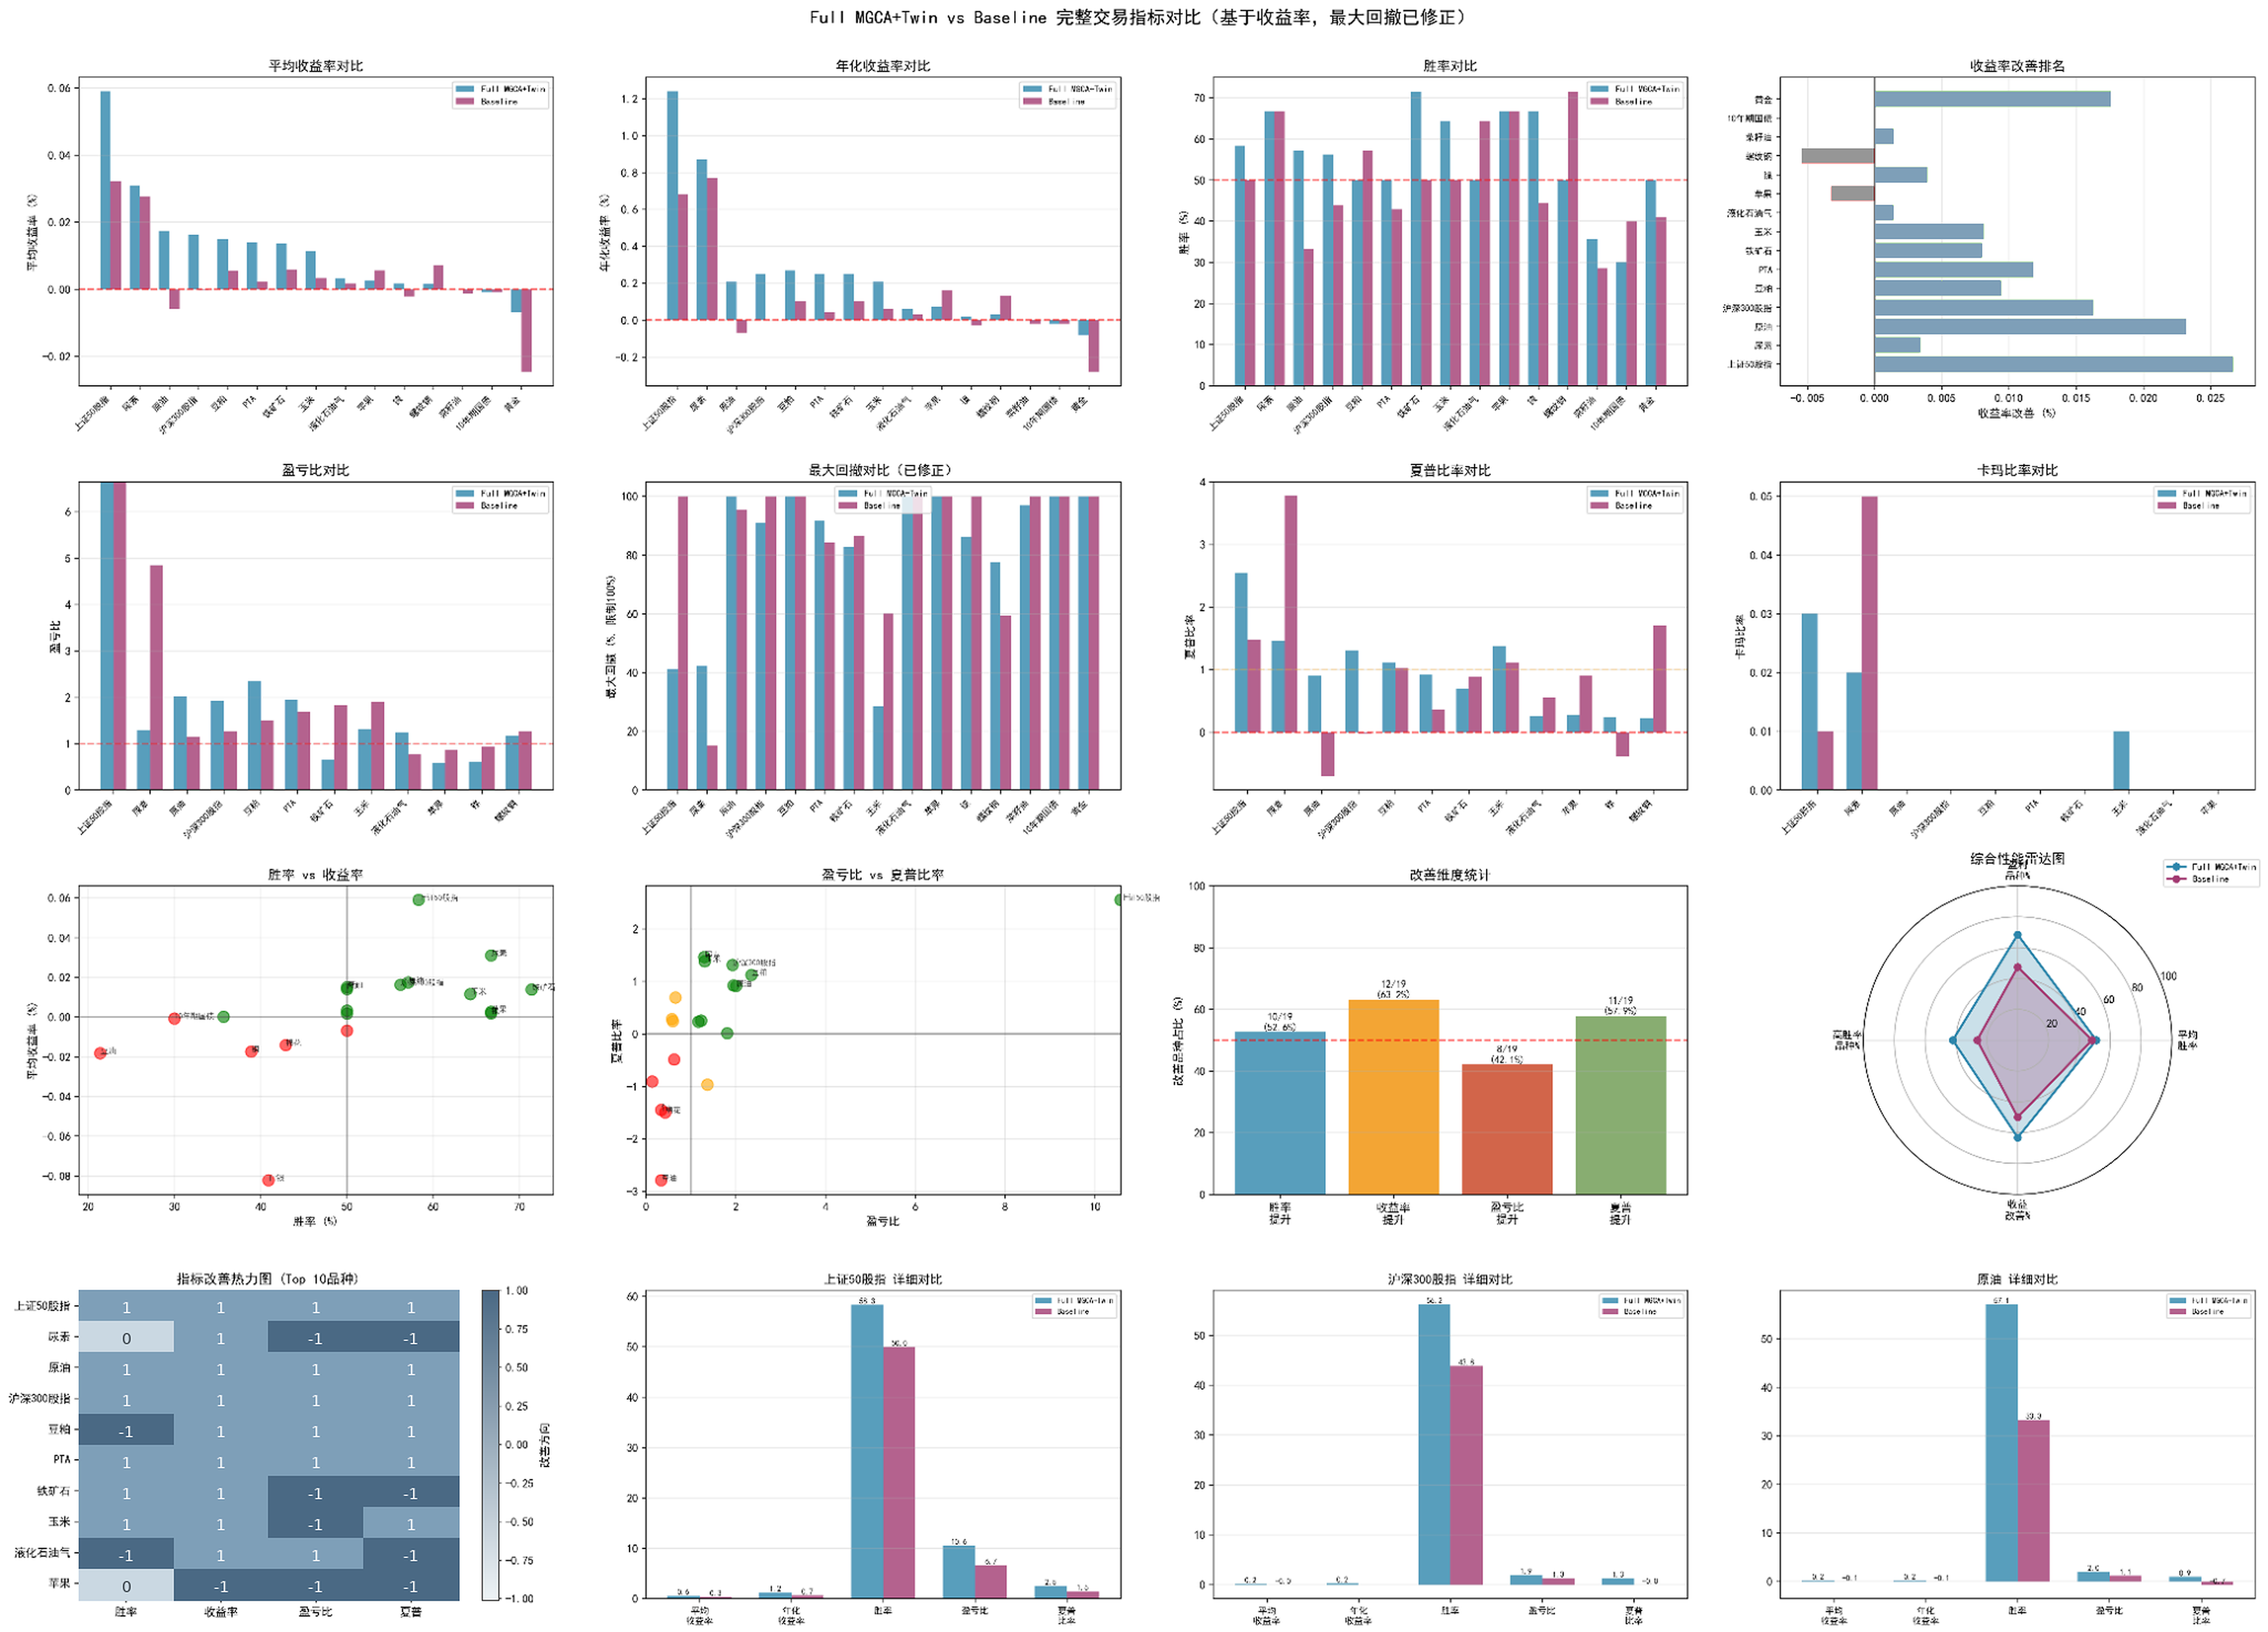
\includegraphics[width=0.96\textwidth]{figures/chap6/图5.13改.png}
\caption{孪生对抗框架综合交易指标对比可视化（16个子图综合分析）}
\label{fig:comprehensiveviz_new}
\end{figure}

图\ref{fig:comprehensiveviz_new}综合可视化了收益率、胜率、盈亏比、最大回撤、夏普比率、卡玛比率及改善热力图等结果。可视化结果与前述表格一致：上证50股指、沪深300股指和原油是多维度改善最明显的代表品种，而部分品种则呈现“某些指标改善、某些指标恶化”的混合特征，也说明执行模型的评价不能只看单一维度。
在多维绩效评价之后，仍需回到交易执行优化的直接目标，即成本改善是否能够在多个品种上稳定出现。表\ref{tab:advanced_performance_new}进一步汇总 19 个品种上的成本节省极值与整体表现，用于观察该机制的跨品种适用性和失效边界。

\FloatBarrier

\begin{table}[!htbp]
\centering
\caption{孪生对抗在19个品种上的成本节省极值与整体表现}
\label{tab:advanced_performance_new}
\small
\setlength{\tabcolsep}{6pt}
\renewcommand{\arraystretch}{1.18}
\begin{tabular}{lcccc}
\toprule
\multirow{2}{*}{\textbf{品种}} & \multicolumn{3}{c}{\textbf{孪生对抗成本(元)}} & \multirow{2}{*}{\makecell{\textbf{基准模型}\\\textbf{成本(元)}}} \\
\cmidrule(lr){2-4}
 & \textbf{平均} & \textbf{最高} & \textbf{最低} &  \\
\midrule
上证50股指 & 15,173 & 88,624 & -6,795 & 8,110 \\
沪深300股指 & 6,047 & 48,403 & -30,672 & -188 \\
10年期国债 & -8 & 95 & -53 & -9 \\
PTA & 6,729 & 92,986 & -40,644 & 1,115 \\
菜籽油 & 1,181 & 221,336 & -107,773 & -820 \\
原油 & 797 & 12,052 & -5,188 & -344 \\
液化石油气 & 1,730 & 56,820 & -58,038 & 832 \\
尿素 & 5,368 & 51,283 & -19,631 & 4,858 \\
铁矿石 & 1,114 & 12,234 & -14,794 & 454 \\
螺纹钢 & 713 & 21,700 & -18,408 & 2,254 \\
豆粕 & 4,660 & 51,155 & -23,239 & 1,672 \\
玉米 & 2,612 & 17,716 & -12,152 & 787 \\
苹果 & 1,431 & 51,264 & -58,590 & 4,456 \\
豆油 & -14,395 & 14,670 & -61,206 & -6,496 \\
棉花 & -18,933 & 78,230 & -140,355 & -7,631 \\
黄金 & -457 & 6,895 & -9,345 & -1,612 \\
白银 & -64,197 & 67,306 & -1,099,435 & -26,781 \\
镍 & 21,592 & 731,412 & -552,995 & -26,469 \\
铜 & -133,553 & 330,227 & -1,261,400 & -17,472 \\
\bottomrule
\end{tabular}
\end{table}
\begin{table}[!htbp]
\centering
{\small\textbf{续表}}\\[0.5em]
\small
\setlength{\tabcolsep}{5pt}
\renewcommand{\arraystretch}{1.18}
\begin{tabular}{lccccc}
\toprule
\multirow{2}{*}{\textbf{品种}} & \multicolumn{3}{c}{\textbf{成本改善(元)}} & \multirow{2}{*}{\makecell{\textbf{均方误差}\\\textbf{变化}}} & \multirow{2}{*}{\makecell{\textbf{盈利率}\\\textbf{(\%)}}} \\
\cmidrule(lr){2-4}
 & \textbf{平均} & \textbf{最高} & \textbf{最低} & & \\
\midrule
上证50股指 & \checkmark +7,063 & +23,753 & -3,398 & +14.0\% & 58.3 \\
沪深300股指 & \checkmark +6,235 & +42,716 & -23,236 & +29.8\% & 56.2 \\
10年期国债 & \checkmark +0 & +29 & -35 & -34.0\% & 30.0 \\
PTA & \checkmark +5,614 & +74,871 & -13,507 & +35.5\% & 50.0 \\
菜籽油 & \checkmark +2,000 & +143,668 & -79,295 & +60.7\% & 35.7 \\
原油 & \checkmark +1,141 & +9,728 & -3,099 & +41.9\% & 57.1 \\
液化石油气 & \checkmark +897 & +45,340 & -45,700 & +67.0\% & 50.0 \\
尿素 & \checkmark +510 & +40,023 & -17,885 & -27.0\% & 66.7 \\
铁矿石 & \checkmark +660 & +10,126 & -10,712 & +58.4\% & 71.4 \\
螺纹钢 & \texttimes -1,541 & +10,082 & -18,219 & -12.1\% & 50.0 \\
豆粕 & \checkmark +2,988 & +32,153 & -16,695 & +107.0\% & 50.0 \\
玉米 & \checkmark +1,825 & +15,342 & -11,063 & +86.9\% & 64.3 \\
苹果 & \texttimes -3,025 & +39,584 & -50,279 & +144.3\% & 66.7 \\
豆油 & \texttimes -7,899 & +47,280 & -153,920 & +34.7\% & 21.4 \\
棉花 & \texttimes -11,302 & +54,508 & -127,654 & +117.9\% & 42.9 \\
黄金 & \checkmark +1,155 & +16,529 & -3,600 & +39.3\% & 50.0 \\
白银 & \texttimes -37,416 & +33,842 & -591,867 & +54.7\% & 40.9 \\
镍 & \checkmark +48,061 & +616,116 & -508,647 & +47.5\% & 66.7 \\
铜 & \texttimes -116,081 & +247,561 & -1,050,160 & +94.9\% & 38.9 \\
\bottomrule
\end{tabular}
\end{table}

表\ref{tab:advanced_performance_new}总结了 19 个品种上的成本节省极值与整体表现。结果显示，13 个品种实现了正向平均成本改善，占比 68.4\%。其中，镍、上证50股指、沪深300股指与 PTA 等中高波动、趋势结构较明显的品种受益更为明显；而铜、白银、豆油等高噪声或博弈较充分的品种则更容易出现执行劣化。这一现象表明，该机制更适合存在非平稳特征但仍保留可辨识微观结构的市场环境。

\FloatBarrier

综合上述结果，可以将本章经验概括为三点。第一，预测精度与执行绩效之间存在非单调关系。部分品种中，孪生对抗的均方误差并不优于基准模型，但在成本节省、收益率与回撤控制上依然取得更好结果，说明执行安全性比均值意义上的统计精度更重要。第二，市场微观结构的适应性具有明显差异。中等波动和中高波动、具有阶段性趋势的品种，更能体现多生成器与孪生纠偏的优势；极低波动或极高噪声品种，则可能分别因为信号不足或噪声过强而削弱收益。第三，自体再生机制的作用主要体现在执行前校验与再平衡环节：它并不保证所有时候都优于基准，但能够在关键阶段过滤异常候选、抑制系统性退化，并为执行系统提供参数恢复路径。

从交易执行优化角度看，本章实验结果的意义不在于证明某一模型在所有品种上都取得最低统计误差，而在于检验孪生对抗自体再生方法是否能够在复杂市场环境中维持执行路径稳定性。本章数据集覆盖多个品种类别和不同波动状态，能够反映成交量分布、流动性条件和价格冲击在真实市场中的差异。若仅以点预测误差评价执行模型，容易忽视关键时点的异常偏离；而在成交量加权平均价格执行任务中，少数关键窗口的错误调度往往会放大为实际滑点和冲击成本。因此，实验解释需要回到执行偏差是否被识别、过滤和优化这一核心问题。

前述表格与曲线显示，孪生对抗自体再生方法的作用主要体现在执行过程的稳定化。一方面，孪生校验和偏离统计使系统能够在候选信号进入最终下单路径前进行筛选，降低明显失真信号直接转化为执行成本的概率；另一方面，跨组修复和短程微调使退化模型能够被及时替换并重新进入可分化的对抗状态，避免局部崩溃继续传导到后续订单切片。因此，本章方法的价值不只在成交量预测层面，而在于把滑点、市场冲击和模型退化纳入同一执行优化过程。成本节省反映执行优化效果，胜率反映下单路径有效性，最大回撤和下行风险则反映执行安全性，这些指标表明交易执行优化不能停留于单一预测误差比较。

当然，实验结果也表明该方法具有适用边界。在极低波动或极高噪声场景下，市场成交量结构本身缺乏稳定可学习模式，孪生校验与再平衡能够提供异常过滤，却不能完全消除市场随机冲击。因此，本章方法更适合作为动态执行系统的安全约束和执行优化模块，而不是替代所有执行决策的单一预测器。
\section{本章小结}

本章围绕对冲基金交易决策流程中的交易执行优化环节，提出面向交易执行优化的孪生对抗自体再生方法，重点服务于交易执行路径优化问题。与第 2 章、第 3 章和第 4 章分别关注投资组合管理、高维金融因子建模和时序结构识别不同，本章进一步关注交易信号进入市场后的执行路径生成、滑点控制和市场冲击约束。该方法的核心并不局限于提高价格或成交量的点预测精度，而是通过“复制—配对—分化”的孪生自体再生逻辑，将执行层面最关键的滑点风险、异常偏离与市场冲击成本内化为可建模、可检测、可触发再平衡的执行优化目标。由此，系统能够在候选执行信号进入最终下单路径前进行孪生校验、偏离识别和动态再平衡，从而降低异常信号直接转化为执行成本的概率。

从真实期货市场的实证结果看，该方法在 19 个代表性品种、279 个 30 分钟成交量加权平均价格执行窗口上表现出一定的跨场景适应性。尽管其在部分品种上的统计拟合精度并不始终优于基准模型，但在成本节省、收益率、胜率、回撤控制与下行风险管理等执行层指标上，整体表现更为稳定。在中高波动且非平稳特征较强的品种上，该方法的市场适应性更为明显；而在极低波动或极高噪声场景下，其效果则受到一定约束。这也表明，评价执行模型不能停留于单一预测误差，而应回到交易成本、执行偏差和风险暴露的经济含义本身。

在市场微观结构频繁变化的条件下，成交量加权平均价格执行效果不仅取决于模型能否给出“平均意义上最接近真实值”的预测，也取决于系统能否在关键节点识别异常、过滤失真并维持相对稳定的执行状态。因此，本章对应交易决策链条中的第四步：在明确资产配置对象选择因子依据形成和交易时机判断之后，进一步讨论交易执行路径优化。通过将预测成交量、执行路径、滑点控制和崩溃修复组织为连续闭环，本章为前序交易信号进入真实成交环节提供执行层支撑。后续第6章将在此基础上面向策略整合，讨论最终交易决策的形成。
